% !TeX spellcheck = pl_PL

%%%%%%%%%%%%%%%%%%%%%%%%%%%%%%%%%%%%%%%%%%%
%                                         %
% Szablon pracy dyplomowej magisterskiej %
%                                         %
%%%%%%%%%%%%%%%%%%%%%%%%%%%%%%%%%%%%%%%%%%%

% Dane autora
\newcommand{\FirstNameAuthor}{Łukasz}
\newcommand{\SurnameAuthor}{Krawczyk}
\newcommand{\IdAuthor}{296657}

% Drugi autor (pozostaw puste, jeśli nie dotyczy)
\newcommand{\FirstNameCoauthor}{}
\newcommand{\SurnameCoauthor}{}
\newcommand{\IdCoauthor}{}

% Promotor
\newcommand{\Supervisor}{Dr inż. Paweł Benecki}

% Tytuł pracy
\newcommand{\Title}{Przekształcanie nagrań dźwiękowych na zapis nutowy}
\newcommand{\TitleAlt}{Converting audio recordings to musical notation}

% Kierunek i specjalność
\newcommand{\Program}{Informatyka}
\newcommand{\Specialisation}{Internet i technologie sieciowe}
\newcommand{\Departament}{Katedra Informatyki Stosowanej}

% Promotor pomocniczy / opiekun (pozostaw puste, jeśli nie dotyczy)
\newcommand{\Consultant}{}

%%%%%%%%%%%%%%%%%%%%%%%%%%%%%%%%%%%%%%%%%%

\input{config/settings.tex}
% Tutaj proszę umieszczać swoje pakiety, makra, ustawienia itd.
%%%%%%%%%%%%%%%%%%%%%%%%%%%%%%%%%%%%%%%%%%%%%%%%%%%%%%%%%%%%%%%%%%%%%
% listingi i fragmentu kodu źródłowego
% pakiet: listings lub minted
% % % % % % % % % % % % % % % % % % % % % % % % % % % % % % % % % % %

% biblioteka listings
\usepackage{listings}
% \usepackage{float} % Było zakomentowane, odkomentowujemy dla opcji [H]
\lstset{%
morekeywords={string,exception,std,vector},% słowa kluczowe rozpoznawane przez pakiet listings
language=C++,% C, Matlab, Python, SQL, TeX, XML, bash, ... – vide https://www.ctan.org/pkg/listings
commentstyle=\textit,%
identifierstyle=\textsf,%
keywordstyle=\sffamily\bfseries, %\texttt, %
%captionpos=b,%
tabsize=3,%
frame=lines,%
numbers=left,%
numberstyle=\tiny,%
numbersep=5pt,%
breaklines=true,%
escapeinside={@*}{*@},%
}


% % % % % % % % % % % % % % % % % % % % % % % % % % % % % % % % % % %
%
% pakiet minted
%\usepackage{minted}

% pakiet wymaga specjalnego kompilowania:
% pdflatex -shell-escape main.tex
% xelatex  -shell-escape main.tex

%\usepackage[chapter]{minted} % [section]
%%\usemintedstyle{bw}   % czarno-białe kody
%
%\setminted % https://ctan.org/pkg/minted
%{
%%fontsize=\normalsize,%\footnotesize,
%%captionpos=b,%
%tabsize=3,%
%frame=lines,%
%framesep=2mm,
%numbers=left,%
%numbersep=5pt,%
%breaklines=true,%
%escapeinside=@@,%
%}

%%%%%%%%%%%%%%%%%%%%%%%%%%%%%%%%%%%%%%%%%%%%%%%%%%%%%%%%%%%%%%%%%%%%%
% Dodano pakiet longtable dla tabel wielostronicowych
\usepackage{longtable}

% OPCJONALNIE: Pakiet float dla lepszej kontroli nad pozycjonowaniem obiektów pływających (opcja [H])
% Odkomentowujemy, aby opcja [H] dla rysunków działała poprawnie
\usepackage{float}

% Dodano pakiet microtype dla lepszego łamania tekstu i justowania
\usepackage{microtype}

% Zapobieganie rozciąganiu pionowych odstępów w celu wypełnienia strony
% Strony będą miały wyrównanie do góry, dolna krawędź może być nierówna.
\raggedbottom

% OPCJONALNIE: Zwiększenie kar za "wdowy" i "sieroty"
% Może pomóc w zmianie sposobu łamania stron, co czasami rozwiązuje problemy z odstępami.
% Możesz to odkomentować, jeśli \raggedbottom samo w sobie nie wystarczy lub jeśli
% chcesz unikać \raggedbottom i szukać innego rozwiązania.
% \clubpenalty=10000 % Kara za "sierotę" (pierwsza linia akapitu na końcu strony)
% \widowpenalty=10000 % Kara za "wdowę" (ostatnia linia akapitu na początku strony)
% \displaywidowpenalty=10000 % Kara za "wdowę" przed formułą matematyczną

% OPCJONALNIE: Pakiet enumitem dla lepszej kontroli nad odstępami w listach
% Jeśli odstępy w listach itemize/enumerate są zbyt duże, można odkomentować:
% \usepackage{enumitem}
% Przykłady konfiguracji (umieścić PO \usepackage{enumitem}):
% \setlist[itemize]{noitemsep} % usuwa odstępy między elementami listy, zachowuje odstęp przed/po liście
% \setlist[itemize]{nosep} % usuwa większość pionowych odstępów w listach itemize
% lub bardziej szczegółowo:
% \setlist[itemize,1]{topsep=5pt, partopsep=2pt, itemsep=2pt, parsep=2pt} % dla pierwszego poziomu zagnieżdżenia
%%%%%%%%%%%%%%%%%%%%%%%%%%%%%%%%%%%%%%%%%%%%%%%

%%%%%%%%%%%%%%%%%%%%%%%%%%%%%%%%%%%%%%%%

\begin{document}

\frontmatter
\input{config/titlepage.tex}

\cleardoublepage
\rmfamily\normalfont
\pagestyle{empty}

% Informacje redakcyjne
\subsubsection*{Tytuł pracy}
\Title{Przekształcanie nagrań dźwiękowych na zapis nutowy}

\subsubsection*{Streszczenie}
Niniejsza praca magisterska porusza problematykę przekształcania nagrań dźwiękowych na zapis nutowy, skupiając się na szczegółowym przypadku automatycznej transkrypcji polifonicznych nagrań gitarowych na zapis tabulaturowy (GTT). W ramach pracy zaprojektowano, zaimplementowano i~zweryfikowano eksperymentalnie system oparty na architekturze konwolucyjno-rekurencyjnej sieci neuronowej (CRNN), która uczy się bezpośredniego mapowania z~reprezentacji czasowo-częstotliwościowej sygnału audio na symboliczną postać tabulatury. Kluczowym elementem projektu jest wielozadaniowe uczenie, w~którym model jednocześnie przewiduje momenty rozpoczęcia dźwięków (onsets) oraz numery aktywnych progów na poszczególnych strunach gitary.

Proces badawczy, przeprowadzony na publicznie dostępnym zbiorze danych GuitarSet, obejmował ponad 70 iteracyjnych eksperymentów. Wykazały one, że decydujący wpływ na skuteczność modelu miała innowacyjna strategia intensywnej augmentacji danych, symulująca niedoskonałości nagrań realizowanych w~warunkach amatorskich, takie jak pogłos, szum czy zniekształcenia mikrofonowe. Zastosowanie tej data-centrycznej strategii pozwoliło na osiągnięcie wyników przewyższających aktualny stan wiedzy.

Finalny model, oceniany na zbiorze testowym, uzyskał wynik MPE F1-Score na poziomie 0.8736, co jest wynikiem lepszym od rezultatów raportowanych w~kluczowych publikacjach w~tej dziedzinie dla modeli trenowanych wyłącznie na zbiorze GuitarSet. Analiza jakościowa potwierdziła wysoką zdolność modelu do poprawnej estymacji wysokości dźwięków, jednocześnie wskazując, że głównym pozostałym wyzwaniem jest precyzyjne rozwiązywanie problemu wieloznaczności opalcowania, wynikającego z~trudności w~klasyfikacji subtelnych różnic w~barwie dźwięku między strunami. Praca dowodzi, że opracowane rozwiązanie stanowi skuteczną i~obiecującą metodę dla GTT, otwierając nowe kierunki dalszych badań.

\subsubsection*{Słowa kluczowe}
przekształcanie sygnału audio, automatyczna transkrypcja muzyczna, notacja muzyczna, transkrypcja gitary, tabulatura

\subsubsection*{Thesis title}
\begin{otherlanguage}{british}
\TitleAlt{Transforming Audio Recordings into Musical Notation}
\end{otherlanguage}

\subsubsection*{Abstract}
\begin{otherlanguage}{british}
This master's thesis addresses the problem of transforming audio recordings into musical notation, focusing on the specific case of automatic transcription of polyphonic guitar recordings into tablature notation (GTT). The project involved the design, implementation, and experimental verification of a system based on a Convolutional Recurrent Neural Network (CRNN) architecture, which learns to directly map a time-frequency representation of an audio signal to a symbolic tablature format. A key element of the project is multi-task learning, where the model simultaneously predicts note onsets and the corresponding fret numbers on individual guitar strings.

The research process, conducted on the publicly available GuitarSet dataset, comprised over 70 iterative experiments. These revealed that the decisive factor for the model's effectiveness was an innovative and aggressive data augmentation strategy. This strategy simulated imperfections of amateur recordings, such as reverb, noise, and microphone distortions. The application of this data-centric approach led to results surpassing the current state-of-the-art.

The final model, evaluated on the test set, achieved an MPE F1-Score of 0.8736, which is superior to results reported in key publications for models trained exclusively on the GuitarSet dataset. Qualitative analysis confirmed the model's high accuracy in pitch estimation, while also indicating that the main remaining challenge is the precise resolution of fingering ambiguity, stemming from the difficulty in classifying subtle timbre differences between strings. The thesis demonstrates that the developed solution constitutes an effective and promising method for GTT, opening new avenues for future research.
\end{otherlanguage}

\subsubsection*{Key words}
\begin{otherlanguage}{british}
audio signal processing, automatic music transcription, music notation, guitar transcription, tablature
\end{otherlanguage}


% Spis treści
\addtocontents{toc}{\protect\thispagestyle{empty}}
\tableofcontents

\setcounter{stronyPozaNumeracja}{\value{page}}
\mainmatter
\pagestyle{empty}
\cleardoublepage
\pagestyle{NumeryStronNazwyRozdzialow}

% Rozdziały pracy
\chapter{Wstęp}
\label{chap:wstep}

Automatyczna Transkrypcja Muzyczna (ATM) (\english{Automatic Music Transcription}) stanowi jedno z kluczowych i jednocześnie najbardziej złożonych zadań w dziedzinie komputerowej analizy muzyki.
W swej istocie, ATM jest procesem konwersji sygnału akustycznego, będącego fizyczną manifestacją muzyki, na jego symboliczną, strukturalną reprezentację \autocite{KlapuriDavy2006SignalProcessing,Benetos2019AutomaticMusicTranscription}.
Celem tego procesu jest przekształcenie ciągłego sygnału audio w dyskretny zestaw symboli muzycznych, takich jak tradycyjne nuty określające wysokość i czas trwania dźwięku, lub – co jest przedmiotem szczególnego zainteresowania w niniejszej pracy – w zapis tabulaturowy.
Interdyscyplinarny charakter Automatycznej Transkrypcji Muzycznej jest niezaprzeczalny, gdyż skuteczna realizacja jej zadań wymaga integracji wiedzy i metodologii pochodzących z wielu, pozornie odległych, dziedzin nauki i techniki.
Do najważniejszych z nich należą:
\begin{itemize}
\item \textbf{Cyfrowe Przetwarzanie Sygnałów (CPS)} (\english{Digital Signal Processing – DSP}): Dostarcza ono fundamentalnych narzędzi do analizy, transformacji i manipulacji sygnałem audio w dziedzinie czasu i częstotliwości.
Techniki takie jak filtracja, analiza spektralna czy transformacje czasowo-częstotliwościowe są nieodzowne w procesie ekstrakcji informacji z surowego sygnału dźwiękowego \autocite{KlapuriDavy2006SignalProcessing}.
Zaawansowane metody CPS pozwalają na wstępne przygotowanie sygnału, redukcję szumów oraz identyfikację podstawowych cech akustycznych, które następnie mogą być interpretowane w kontekście muzycznym.
Przykładem fundamentalnego narzędzia CPS, ilustrującego przejście z dziedziny czasu do dziedziny częstotliwości, jest dyskretna transformata Fouriera (DFT) (\english{Discrete Fourier Transform}).
Dla skończonego ciągu próbek sygnału $x_n$ o długości N, jej k-ty współczynnik $X_k$ jest zdefiniowany jako:
\begin{equation}
X_k = \sum_{n=0}^{N-1} x_n \cdot e^{-i\frac{2\pi}{N}kn}
\label{eq:dft}
\end{equation}
gdzie $n$ jest indeksem próbki w dziedzinie czasu, $k$ jest indeksem częstotliwości, a $i$ jest jednostką urojoną.
Wzór ten jest podstawą wielu algorytmów analizy częstotliwościowej stosowanych w ATM.
\item \textbf{Rozpoznawanie Wzorców} (\english{Pattern Recognition}) oraz \textbf{Uczenie Maszynowe (UM)} (\english{Machine Learning – ML}): Te dziedziny odgrywają kluczową rolę w identyfikacji złożonych struktur muzycznych, takich jak pojedyncze nuty, akordy, rytmy czy motywy melodyczne, w często zaszumionym i polifonicznym sygnale audio \autocite{Benetos2019AutomaticMusicTranscription}.
Współczesne systemy ATM w coraz większym stopniu opierają się na zaawansowanych modelach uczenia maszynowego, w szczególności na sieciach neuronowych i głębokim uczeniu (\english{Deep Learning}), które potrafią automatycznie uczyć się hierarchicznych reprezentacji cech muzycznych bezpośrednio z danych \autocite{BurletHindle2017IsolatedGuitarTranscription}.
Dynamiczny rozwój w obszarze głębokiego uczenia bezpośrednio przekłada się na postępy w ATM, umożliwiając tworzenie modeli zdolnych do przetwarzania coraz bardziej skomplikowanych sygnałów muzycznych z niespotykaną dotąd dokładnością.
\item \textbf{Sztuczna Inteligencja (SI)} (\english{Artificial Intelligence – AI}): Jako szersza dziedzina, obejmuje ona uczenie maszynowe, ale także inne aspekty, takie jak reprezentacja wiedzy muzycznej oraz procesy poznawcze związane z percepcją i wnioskowaniem w kontekście muzycznym \autocite{Benetos2019AutomaticMusicTranscription}.
Rozwój SI dostarcza ram koncepcyjnych i narzędziowych dla budowy inteligentnych systemów transkrypcji.
\item \textbf{Muzykologia}: Dostarcza niezbędnej wiedzy teoretycznej o strukturze muzyki, notacji, harmonii, rytmie oraz praktykach wykonawczych \autocite{Holzapfel2019Ethnomusicology}.
Zrozumienie zasad muzycznych jest kluczowe nie tylko dla interpretacji wyników generowanych przez systemy ATM, ale również dla projektowania algorytmów, które uwzględniają kontekst muzyczny i dążą do tworzenia transkrypcji użytecznych z perspektywy muzykologicznej i wykonawczej.
\end{itemize}

Potencjalne obszary zastosowań systemów ATM są szerokie i różnorodne, co podkreśla ich rosnące znaczenie zarówno w badaniach naukowych, jak i w praktyce muzycznej.
Do najważniejszych aplikacji należą: wsparcie w edukacji muzycznej, na przykład poprzez tworzenie systemów do automatyzacji ćwiczeń gry na instrumencie, analizę postępów ucznia czy generowanie spersonalizowanych materiałów dydaktycznych \autocite{Benetos2019AutomaticMusicTranscription}.
Systemy ATM mogą również znacząco ułatwić proces tworzenia i aranżacji muzyki, na przykład poprzez wspieranie modyfikacji i rearanżacji istniejących utworów \autocite{ArndtLi2012AutomatedTranscription}.
Dla producentów muzycznych, ATM oferuje narzędzia do wizualizacji treści muzycznej i inteligentnej edycji nagrań \autocite{Benetos2019AutomaticMusicTranscription}.
Ponadto, technologie te są wykorzystywane w systemach wyszukiwania i kategoryzacji muzyki w dużych zbiorach danych, na przykład poprzez umożliwienie wyszukiwania utworów na podstawie ich melodii, harmonii czy rytmu \autocite{Benetos2019AutomaticMusicTranscription}.
Tytuł niniejszej pracy, ,,Przekształcanie nagrań dźwiękowych na zapis nutowy'', odnosi się do centralnego problemu ATM.
Należy jednak podkreślić, że termin ,,zapis nutowy'' jest pojęciem szerokim, obejmującym różnorodne systemy notacji muzycznej.
W kontekście niniejszego opracowania, szczególna uwaga zostanie poświęcona specyficznej formie zapisu, jaką jest tabulatura gitarowa.
Tabulatura, w odróżnieniu od tradycyjnej notacji nutowej skupiającej się \english{primarnie} na wysokości i czasie trwania dźwięku, jest graficzną reprezentacją wskazującą bezpośrednio pozycje palców na gryfie instrumentu – konkretne struny i progi, które należy nacisnąć, aby uzyskać pożądany dźwięk \autocite{Wiggins2019TabCNN}.
\begin{figure}[htbp]
\centering
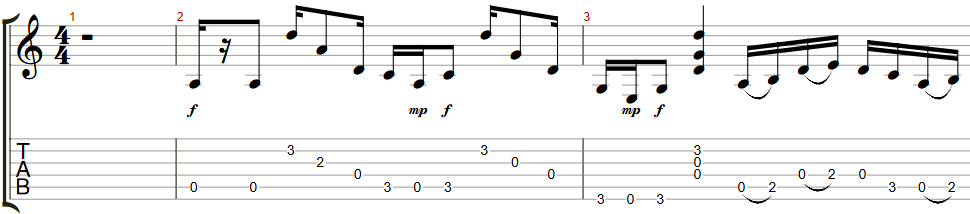
\includegraphics[width=0.9\textwidth]{fig/fig_1_1.png}
\caption{Porównanie fragmentu zapisu nutowego i odpowiadającej mu tabulatury gitarowej dla motywu muzycznego.}
\label{fig:porownanie_nuty_tabulatura}
\end{figure}

Wybór tabulatury jako docelowej formy zapisu w tej pracy nie jest przypadkowy.
Wynika on ze specyfiki gitary jako instrumentu oraz z ogromnej popularności tej formy notacji wśród gitarzystów \autocite{Wiggins2019TabCNN}.
Rosnąca popularność tabulatur, często udostępnianych online, stwarza specyficzne zapotrzebowanie na systemy ATM zdolne do generowania tego właśnie formatu.
Nie jest to jedynie kwestia preferencji użytkowników; tabulatura często zawiera informacje o charakterze performatywnym, takie jak konkretne opalcowanie czy użycie technik gitarowych, których brakuje w standardowej notacji nutowej.
Skuteczne systemy ATM generujące tabulatury mogą zatem zdemokratyzować proces nauki gry na gitarze oraz tworzenia muzyki, obniżając barierę wejścia dla osób, które nie posługują się biegle tradycyjnym zapisem nutowym, ale rozumieją intuicyjny charakter tabulatury.
Ten wybór stanowi naturalne przejście do dalszych, bardziej szczegółowych rozważań przedstawionych w kolejnych rozdziałach pracy.

\section{Osadzenie problemu w dziedzinie naukowej}
\label{sec:osadzenie_problemu}

Przedmiotem niniejszej pracy jest zagadnienie automatycznej transkrypcji muzyki gitarowej do postaci tabulatury, co sytuuje ją w szerokim kontekście badań prowadzonych w ramach dziedziny naukowej znanej jako \english{Music Information Retrieval (MIR)}.
MIR, czyli komputerowe pozyskiwanie informacji muzycznej, jest interdyscyplinarnym polem badawczym zajmującym się analizą, przetwarzaniem, wyszukiwaniem, organizacją i dostępem do informacji zawartej w muzyce, zarówno w jej formie akustycznej, jak i symbolicznej.
Obserwowany w ostatnich dekadach gwałtowny wzrost ilości dostępnych cyfrowych treści muzycznych, na przykład w ramach cyfrowych bibliotek muzycznych i serwisów streamingowych \autocite{Benetos2019AutomaticMusicTranscription}, generuje rosnące zapotrzebowanie na zautomatyzowane narzędzia do ich analizy.
Narzędzia te są niezbędne do efektywnego zarządzania ogromnymi repozytoriami muzyki, ich przeszukiwania, kategoryzacji oraz personalizacji dostępu dla użytkowników.
ATM jest jednym z kluczowych zadań w ramach MIR, umożliwiającym transformację sygnału audio na bogatszą, symboliczną reprezentację, która może być dalej przetwarzana i analizowana.
Szczególną uwagę w kontekście niniejszej pracy należy poświęcić wyzwaniom związanym z transkrypcją muzyki gitarowej.
Gitara, będąca instrumentem niezwykle popularnym i wszechstronnym, wykorzystywanym w niemal każdym gatunku muzycznym, stawia przed systemami ATM szereg specyficznych trudności:
\begin{itemize}
\item \textbf{Polifoniczność}: Gitara jest instrumentem polifonicznym, co oznacza zdolność do jednoczesnego wydawania wielu dźwięków (standardowo do sześciu, po jednym na każdej strunie) \autocite{BurletHindle2017IsolatedGuitarTranscription}.
Nakładanie się składowych harmonicznych wielu jednocześnie brzmiących dźwięków w sygnale audio znacząco komplikuje proces ich separacji i identyfikacji.
\begin{figure}[htbp]
\centering
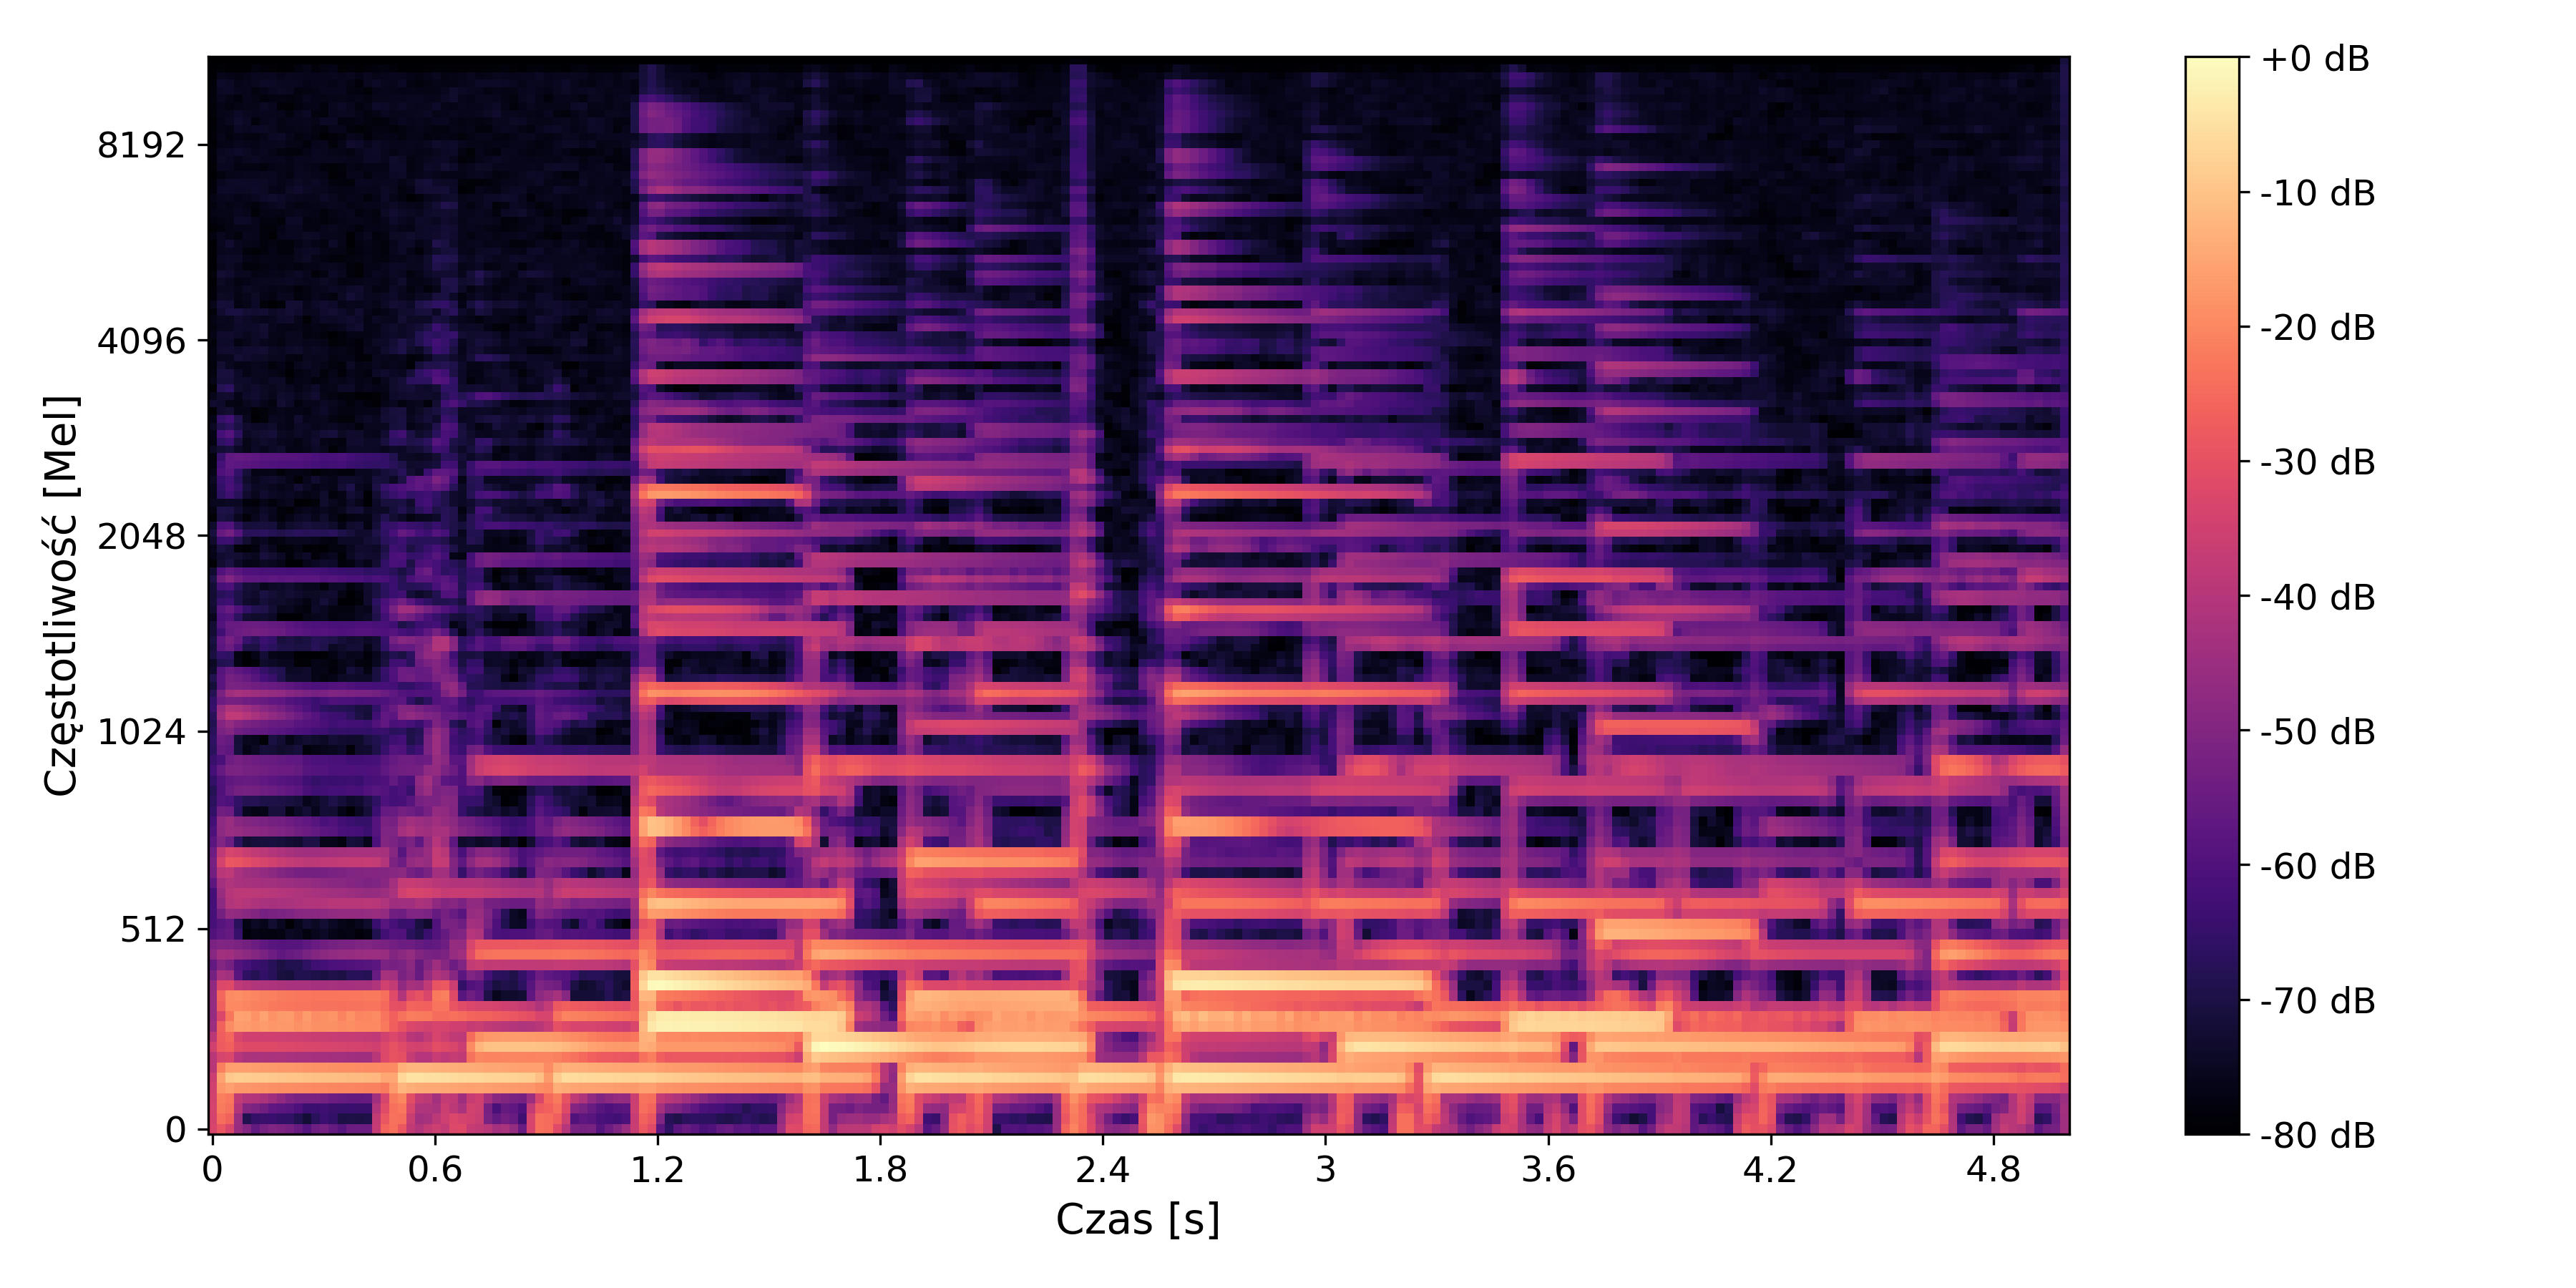
\includegraphics[width=\textwidth]{fig/fig_1_2.png}
\caption{Schematyczny przykład spektrogramu polifonicznego sygnału gitarowego, ukazujący nakładające się struktury harmoniczne (prążki reprezentujące częstotliwość podstawową i jej alikwoty) dla kilku jednocześnie brzmiących nut.}
\label{fig:spektrogram_polifoniczny}
\end{figure}
\item \textbf{Bogactwo technik artykulacyjnych}: Gitarzyści wykorzystują szeroki wachlarz technik artykulacyjnych, takich jak podciąganie strun (\english{bending}), ślizgi (\english{sliding}), młoteczkowanie (\english{hammer-on}), odrywanie (\english{pull-off}), wibrato (\english{vibrato}) czy tłumienie strun dłonią (\english{palm-muting}).
Każda z tych technik w unikalny sposób modyfikuje charakterystykę sygnału akustycznego (np. jego wysokość, amplitudę, barwę w czasie) i jest kluczowa dla wiernej transkrypcji, zwłaszcza do formatu tabulatury, który często zawiera symbole oznaczające te techniki.
\item \textbf{Duża zmienność barwy dźwięku (\english{timbre})}: Barwa dźwięku gitary jest niezwykle zróżnicowana i zależy od wielu czynników, takich jak typ instrumentu (np. gitara akustyczna, klasyczna, elektryczna), rodzaj użytych strun, sposób ich pobudzenia (kostką, palcami), a w przypadku gitar elektrycznych – od ustawień wzmacniacza i zastosowanych efektów gitarowych \autocite{Wiggins2019TabCNN}.
Ta duża wariabilność barwy stanowi poważne wyzwanie dla modeli uczenia maszynowego, które muszą generalizować swoją wiedzę na różne instancje dźwięków gitarowych.
\item \textbf{Identyczność wysokości dźwięku na różnych strunach i progach}: Jedną z charakterystycznych cech gitary jest możliwość zagrania dźwięku o tej samej wysokości w wielu różnych pozycjach na gryfie (tj. na różnych kombinacjach struny i progu) \autocite{Wiggins2019TabCNN}.
O ile dla tradycyjnej notacji nutowej ta wieloznaczność nie jest problemem, o tyle dla generowania tabulatury, która musi precyzyjnie wskazać miejsce zagrania dźwięku, jest to fundamentalne wyzwanie.
Wybór odpowiedniej pozycji często zależy od kontekstu muzycznego, grywalności (łatwości wykonania) i preferencji wykonawcy.
\end{itemize}

Pomimo znaczących postępów, jakie dokonały się w dziedzinie ATM w ostatnich latach, zwłaszcza dzięki zastosowaniu zaawansowanych technik uczenia maszynowego, istniejące systemy wciąż borykają się z ograniczeniami, prowadzącymi do typowych błędów, takich jak pomyłki oktawowe, niepoprawne detekcje nut czy niedokładności czasowe \autocite{Benetos2019AutomaticMusicTranscription}.
Człowiek, dokonując transkrypcji, opiera się nie tylko na percepcji sygnału akustycznego, ale również na swojej rozległej wiedzy muzycznej, znajomości teorii muzyki, konwencji stylistycznych oraz kontekstu kulturowego.
Maszyny, mimo coraz doskonalszych algorytmów, wciąż mają trudności z pełnym uwzględnieniem tych aspektów \autocite{Holzapfel2019Ethnomusicology}.
Ograniczenia te są szczególnie widoczne w przypadku transkrypcji muzyki polifonicznej, wykonywanej na instrumentach o złożonej charakterystyce akustycznej, takich jak gitara \autocite{BurletHindle2017IsolatedGuitarTranscription}.
Niedoskonałość obecnych systemów, zwłaszcza w kontekście precyzyjnego odwzorowania niuansów wykonawczych gitary i generowania użytecznych, grywalnych tabulatur, stanowi silny impuls do poszukiwania nowych, bardziej efektywnych rozwiązań.
Ta luka badawcza jest główną motywacją do podjęcia tematu niniejszej pracy.
Popularność gitary oraz ogromna ilość dostępnych nagrań gitarowych, często pozbawionych wiarygodnych transkrypcji, tworzą naturalne zapotrzebowanie na narzędzia MIR, w tym ATM.
Postępy w tej dziedzinie mogą z kolei stymulować dalsze tworzenie i udostępnianie muzyki, tworząc pozytywną pętlę sprzężenia zwrotnego.
Co więcej, rozwój precyzyjnych systemów ATM dla gitary może odegrać istotną rolę w dokumentacji i archiwizacji unikalnych stylów gitarowych oraz technik wykonawczych, stanowiących ważne elementy dziedzictwa kulturowego.
Otwartym problemem pozostaje również ocena jakości transkrypcji, zwłaszcza w kontekście tabulatur, co zostało zasygnalizowane w literaturze \autocite{Zang2023SynthTab}.

\section{Cel pracy}
\label{sec:cel_pracy}

Głównym celem niniejszej pracy magisterskiej jest zaprojektowanie, implementacja oraz weryfikacja eksperymentalna systemu służącego do automatycznej transkrypcji polifonicznych nagrań audio gitary na zapis tabulaturowy.
Kluczowym elementem realizacji tego celu jest wykorzystanie publicznie dostępnego zbioru danych Guitarset.
Zbiór ten, opisany i wykorzystany w badaniach nad transkrypcją gitarową (np. \autocite{Wiggins2019TabCNN}), został specjalnie przygotowany do tego celu i charakteryzuje się unikalnymi cechami, takimi jak dostarczanie nagrań heksafonicznych (sygnału z każdej struny osobno) wraz z precyzyjnymi adnotacjami dotyczącymi wysokości dźwięku, czasu jego trwania oraz, co szczególnie istotne, informacji o strunie i progu, na którym dany dźwięk został zagrany \autocite{Wiggins2019TabCNN}.
Wybór zbioru Guitarset jest zatem nieprzypadkowy; jego struktura bezpośrednio adresuje problem niejednoznaczności przypisania dźwięku do konkretnej pozycji na gryfie, co jest fundamentalne przy tworzeniu wiarygodnych danych uczących i testowych dla zadania generowania tabulatury.
System opracowany w ramach tej pracy ma dążyć do precyzyjnego odwzorowania partii gitarowych w formie tabulatury.
Oznacza to nie tylko poprawną identyfikację atrybutów muzycznych takich jak wysokość i czas trwania dźwięków, ale przede wszystkim ich prawidłowe przypisanie do odpowiednich strun i progów na gryfie gitary.
Dążenie do precyzji obejmuje również próbę radzenia sobie z wyzwaniami specyficznymi dla transkrypcji gitary, które zostały omówione w poprzednim podrozdziale, takimi jak wysoki stopień polifonii, zróżnicowane techniki artykulacyjne oraz konieczność generowania tabulatury uwzględniającej aspekty grywalności.
Realizacja tak zdefiniowanego celu pracy, czyli stworzenie efektywnego systemu transkrypcji nagrań gitarowych do postaci tabulatury, może przyczynić się do powstania nowych narzędzi wspierających kreatywność i edukację gitarzystów.
Przykładowo, taki system mógłby służyć do automatycznego generowania tabulatur z improwizowanych fragmentów muzycznych, ułatwiać analizę złożonych partii gitarowych znanych wykonawców, czy też stanowić cenne wsparcie w procesie nauki gry na instrumencie.

\section{Zakres pracy}
\label{sec:zakres_pracy}

Realizacja postawionego celu badawczego obejmuje następujące, kluczowe etapy:
\begin{itemize}
\item Przeprowadzenie szczegółowej analizy literatury naukowej dotyczącej automatycznej transkrypcji muzycznej, ze szczególnym naciskiem na metody stosowane w transkrypcji muzyki gitarowej, specyfikę sygnału generowanego przez ten instrument oraz różne aspekty notacji tabulaturowej, w tym jej strukturę i konwencje zapisu.
\item Zaprojektowanie architektury systemu do automatycznej transkrypcji, która będzie uwzględniać specyfikę zadania, charakterystykę danych wejściowych (polifoniczne nagrania gitary akustycznej) i wyjściowych (zapis tabulaturowy) oraz dostępne narzędzia i technologie, w tym potencjalne wykorzystanie modeli głębokiego uczenia.
\item Implementacja kluczowych modułów składowych systemu, obejmujących co najmniej:
\begin{itemize}
\item Moduł przetwarzania wstępnego sygnału audio (\english{audio preprocessing}), mający na celu przygotowanie sygnału do dalszej analizy, np. poprzez normalizację, segmentację czy redukcję szumów.
\item Moduł ekstrakcji cech akustycznych (\english{acoustic feature extraction}), odpowiedzialny za przekształcenie przetworzonego sygnału audio w reprezentację numeryczną, która efektywnie koduje informacje istotne dla rozpoznawania dźwięków gitarowych i ich atrybutów.
Rozważone zostaną zarówno klasyczne cechy akustyczne \autocite{KlapuriDavy2006SignalProcessing}, jak i cechy uzyskiwane automatycznie z wykorzystaniem metod głębokiego uczenia \autocite{BurletHindle2017IsolatedGuitarTranscription}.
\item Moduł predykcyjny, oparty na wybranych technikach uczenia maszynowego, którego zadaniem będzie generowanie sekwencji zdarzeń tabulatu\-rowych (struna, próg, czas rozpoczęcia, czas trwania) na podstawie wyekstra\-howanych cech akustycznych.
\end{itemize}
\item Adaptacja i wykorzystanie publicznie dostępnego zbioru danych Guitarset, opisanego m.in. w \autocite{Wiggins2019TabCNN}, do procesu trenowania, walidacji oraz testowania opracowanego systemu.
Etap ten będzie obejmował przygotowanie danych do formatu wymaganego przez zaimplementowany model, w tym potencjalne techniki augmentacji danych w celu zwiększenia robustości modelu.
\item Zdefiniowanie i dobór odpowiednich metryk oceny jakości transkrypcji tabulaturowej.
Metryki te muszą uwzględniać nie tylko poprawność wykrytych nut pod względem ich wysokości, czasu rozpoczęcia i czasu trwania, ale także, co kluczowe dla tego zadania, poprawność przypisania poszczególnych dźwięków do konkretnych strun i progów gitary.
\item Przeprowadzenie kompleksowych badań eksperymentalnych mających na celu weryfikację skuteczności i wydajności zaproponowanego rozwiązania.
Wyniki uzyskane przez system będą porównywane z adnotacjami referencyjnymi ze zbioru Guitarset oraz, w miarę możliwości, z wynikami innych istniejących metod lub systemów transkrypcji gitarowej, aby ocenić postęp względem aktualnego stanu wiedzy (\english{state-of-the-art}) \autocite{Benetos2019AutomaticMusicTranscription}.
\item Dokładna analiza uzyskanych wyników eksperymentalnych, obejmująca zarówno ocenę ilościową (na podstawie zdefiniowanych metryk), jak i jakościową (np. poprzez analizę typowych błędów popełnianych przez system).
Na tej podstawie zostaną zidentyfikowane mocne i słabe strony opracowanego systemu oraz sformułowane wnioski końcowe i rekomendacje dotyczące potencjalnych ulepszeń oraz dalszych kierunków badań w tej dziedzinie.
\end{itemize}
Niniejsza praca będzie koncentrować się na rozwiązaniu konkretnego problemu o charakterze naukowo-badawczym.
Osiągnięcie tego celu nastąpi poprzez opracowanie innowacyjnego rozwiązania technicznego, jakim jest system do automatycznej transkrypcji gitarowej na tabulaturę, oraz udokumentowanie kompetencji inżynierskich autora w zakresie projektowania, implementacji i weryfikacji systemów opartych na przetwarzaniu sygnałów i uczeniu maszynowym.
Przedstawiony zakres pracy odzwierciedla standardowy cykl życia projektu badawczo-rozwojowego w dziedzinie uczenia maszynowego, co zapewnia metodyczne i kompleksowe podejście do postawionego problemu.
Szczególny nacisk położony na adaptację zbioru Guitarset oraz zdefiniowanie specyficznych metryk oceny jakości transkrypcji tabulaturowej wskazuje na potencjalny wkład pracy nie tylko w sam system, ale również w metodykę badań nad transkrypcją gitarową.

\section{Zwięzła charakterystyka rozdziałów}
\label{sec:charakterystyka_rozdzialow}

Struktura niniejszej pracy magisterskiej została zaprojektowana w sposób umożliwiający logiczne i spójne przedstawienie podjętej problematyki, przeprowadzonych badań oraz uzyskanych wyników.
Poniżej przedstawiono zwięzłą charakterystykę poszczególnych rozdziałów:
\begin{description}
\item[Rozdział 1 (Wstęp)] Prezentowany rozdział. Wprowadza on w problematykę pracy, definiuje automatyczną transkrypcję muzyczną (ATM) i jej specyfikę w kontekście gitary i tabulatury.
Osadza problem w dziedzinie naukowej \english{Music Information Retrieval (MIR)}, omawia wyzwania związane z transkrypcją gitarową.
Formułuje cel i zakres pracy, przedstawia strukturę kolejnych rozdziałów oraz jednoznacznie określa wkład autora.
\item[Rozdział 2 (Analiza Tematu)] Rozdział ten poświęcony będzie dogłębnemu przedstawieniu podstaw teoretycznych niezbędnych do zrozumienia problematyki pracy.
Omówione zostaną fundamentalne pojęcia dotyczące dźwięku muzycznego, jego cyfrowej reprezentacji \autocite{KlapuriDavy2006SignalProcessing} oraz podstawowych metod jego analizy.
Następnie, zaprezentowane zostaną ogólne zagadnienia związane z automatyczną transkrypcją muzyczną, po czym szczegółowa uwaga zostanie skupiona na specyfice transkrypcji gitarowej.
Dokładnie scharakteryzowany zostanie sygnał gitary, jego cechy akustyczne oraz notacja tabulaturowa.
Rozdział ten płynnie przejdzie do sprecyzowania problematyki badawczej podejmowanej w niniejszej pracy.
\item[Rozdział 3 (Przedmiot Pracy)] W tym rozdziale opisane zostanie autorskie rozwiązanie problemu automatycznej transkrypcji polifonicznych nagrań gitarowych na zapis tabulaturowy.
Zaprezentowana zostanie szczegółowa architektura zaimplementowanego systemu, wraz z opisem poszczególnych jego modułów.
Dokładnie scharakteryzowany zostanie wykorzystany zbiór danych Guitarset, którego cechy i zastosowanie w badaniach opisano m.in. w \autocite{Wiggins2019TabCNN}, oraz proces jego adaptacji na potrzeby systemu. Uzasadniony zostanie również wybór zastosowanych metod przetwarzania sygnału, ekstrakcji cech, algorytmów uczenia maszynowego oraz wykorzystanych narzędzi programistycznych.
\item[Rozdział 4 (Badania)] Ten rozdział będzie poświęcony prezentacji metodyki oraz wyników przeprowadzonych badań eksperymentalnych.
Opisane zostanie środowisko badawcze, sposób przygotowania danych testowych oraz zdefiniowane metryki oceny jakości transkrypcji.
Uzyskane wyniki zostaną zaprezentowane w sposób ilościowy (np. w postaci tabel i wykresów) oraz jakościowy.
Następnie wyniki te zostaną poddane szczegółowej analizie i dyskusji, w tym identyfikacji typowych błędów popełnianych przez system oraz porównaniu z istniejącymi rozwiązaniami lub stanem wiedzy.
\item[Rozdział 5 (Podsumowanie)] Ostatni rozdział pracy będzie zawierał syntetyczne podsumowanie wszystkich zrealizowanych prac.
Zaprezentowane zostaną kluczowe wnioski końcowe wynikające z przeprowadzonych badań i analiz. Oceniony zostanie stopień realizacji postawionego celu pracy.
Wskazane zostaną również potencjalne kierunki dalszego rozwoju opracowanego systemu oraz możliwe przyszłe badania w tej dziedzinie, być może w nawiązaniu do otwartych problemów i wyzwań identyfikowanych w literaturze.
\end{description}
Przedstawiona struktura pracy jest zgodna ze standar\-dami pisania prac naukowo-badawczych w dziedzinach technicznych, co zapewnia jej spójność i kompletność.
Wyraźne oddzielenie rozdziału poświęconego analizie tematu od rozdziału opisującego przedmiot pracy pozwala na klarowne rozróżnienie między przeglądem istniejącej wiedzy a oryginalnym wkładem autora, co jest kluczowe dla rzetelnej oceny pracy magisterskiej.

\section{Jednoznaczne określenie wkładu autora}
\label{sec:wklad_autora}

W tej części precyzyjnie określony zostaje indywidualny wkład autora w realizację niniejszej pracy.
Obejmuje on następujące kluczowe aspekty, za które autor był samodzielnie odpowiedzialny:
\begin{itemize}
\item Samodzielne przeprowadzenie gruntownych studiów literaturowych oraz krytyczną analizę aktualnego stanu wiedzy i badań w dziedzinie automatycznej transkrypcji muzycznej, ze szczególnym uwzględnieniem problematyki transkrypcji muzyki gitarowej oraz specyfiki zapisu tabulaturowego.
\item Opracowanie oryginalnej koncepcji oraz zaprojektowanie architektury systemu przeznaczonego do automatycznej transkrypcji polifonicznych nagrań gitarowych na postać tabulatury, uwzględniającej specyficzne wyzwania związane z tym zadaniem.
\item Implementacja algorytmów przetwarzania sygnału audio, metod ekstrakcji cech akustycznych oraz modeli uczenia maszynowego, które stanowią rdzeń funkcjonalny opracowanego systemu transkrypcji.
\item Adaptacja, przygotowanie oraz analiza publicznie dostępnego zbioru danych Guitarset na potrzeby procesu trenowania, walidacji i kompleksowej ewaluacji zaprojektowanego i zaimplementowanego systemu.
\item Zaprojektowanie metodyki oraz samodzielne przeprowadzenie kompleksowych badań eksperymentalnych, mających na celu weryfikację skuteczności, wydajności oraz ograniczeń opracowanego rozwiązania w kontekście transkrypcji gitarowej na tabulaturę.
\item Krytyczna analiza i interpretacja uzyskanych wyników eksperymentalnych, w tym identyfikacja mocnych i słabych stron systemu, oraz ocena istotności tych wyników w kontekście istniejących rozwiązań i aktualnego stanu wiedzy w dziedzinie.
\item Sformułowanie wniosków końcowych podsumowujących całość przeprowadzonych prac badawczych i implementacyjnych, a także przedstawienie propozycji dotyczących potencjalnych ulepszeń systemu oraz możliwych kierunków dalszych badań.
\end{itemize}
Powyższe wyszczególnienie ma na celu jednoznaczne wyodrębnienie oryginalnego wkładu studenta w identyfikację i rozwiązanie postawionego problemu badawczego, a także w opracowanie, implementację i weryfikację opisanego systemu informatycznego.
Wymienione punkty pokrywają cały proces badawczy, od fazy koncepcyjnej, poprzez realizację techniczną, aż po analizę wyników i formułowanie wniosków, co świadczy o kompleksowym i samodzielnym charakterze pracy, zgodnie z oczekiwaniami stawianymi pracom magisterskim.
Nacisk na ,,oryginalną koncepcję'' oraz ,,krytyczną analizę'' podkreśla aspiracje pracy do wniesienia wartościowego wkładu w rozwój dziedziny, wykraczającego poza jedynie odtwórcze zastosowanie znanych metod.  % Wstęp
\chapter[Analiza tematu: podstawy i specyfika transkrypcji gitarowej]{Analiza tematu: teoretyczne podstawy transkrypcji muzycznej i specyfika transkrypcji gitarowej}
\label{chap:analiza_tematu}

Rozdział pierwszy wprowadził w~ogólną problematykę automatycznej transkrypcji muzycznej (ATM) oraz zarysował specyficzne wyzwania związane z~muzyką gitarową. Niniejszy rozdział stanowi rozwinięcie podstaw teoretycznych, które są niezbędne do pełnego zrozumienia podejmowanego problemu oraz zaprojektowanego rozwiązania. Skupia się on na szczegółowej analizie dźwięku muzycznego, jego cyfrowej reprezentacji oraz metodach stosowanych w~ATM, kładąc fundament pod dalsze, bardziej techniczne części pracy.

\section{Sprecyzowanie problemu badawczego}
\label{sec:definicja_problemu_atm}

Jak wskazano we wstępie, proces ATM polega na przekształceniu sygnału audio na jego symboliczną reprezentację, taką jak format piano-roll czy standardowy zapis nutowy~\autocite{KlapuriDavy2006SignalProcessing,Benetos2019AutomaticMusicTranscription}. W~kontekście niniejszej pracy, problem ten zostaje sprecyzowany jako \textbf{automatyczna transkrypcja gitarowa na zapis tabulaturowy (GTT)} (ang. \textit{Guitar Tablature Transcription}). Zadanie GTT wykracza poza prostą identyfikację wysokości i~czasu trwania dźwięków, ponieważ obejmuje również ich precyzyjne przypisanie do konkretnych strun i~progów na gryfie gitary~\autocite{Wiggins2019TabCNN}. Ponadto, pełna transkrypcja tabulaturowa dąży do rozpoznania technik artykulacyjnych charakterystycznych dla gitary, takich jak podciągnięcia strun (ang. \textit{bends}), młoteczkowanie (ang. \textit{hammer-on}), odrywanie (ang. \textit{pull-off}) czy wibrato (ang. \textit{vibrato})~\autocite{Reboursiere2011GuitarController}, które są kluczowe dla wiernego odtworzenia utworu.

Mimo znaczącego potencjału aplikacyjnego, należy zauważyć, że obecne systemy ATM mogą nie zawsze oferować przewagę w~każdym scenariuszu, np. w~kontekstach etnomuzykologicznych, gdzie dla doświadczonych transkrybentów krytyczna jest precyzja notacji rytmicznej~\autocite{Holzapfel2019Ethnomusicology}.
\section{Podstawy teoretyczne: dźwięk muzyczny i jego cyfrowa reprezentacja}
\label{sec:podstawy_teoretyczne_dzwiek}

Zrozumienie procesów leżących u~podstaw automatycznej transkrypcji muzycznej wymaga uprzedniego zapoznania się z~właściwościami dźwięku muzycznego oraz sposobami jego cyfrowej reprezentacji i~analizy. Niniejsza sekcja przybliża te kluczowe koncepcje.

\subsection{Percepcyjne i fizyczne atrybuty dźwięku muzycznego}
\label{ssec:atrybuty_dzwieku}

Dźwięk muzyczny, z~perspektywy percepcji, charakteryzowany jest przez cztery podstawowe atrybuty: wysokość, głośność, barwę i~czas trwania~\autocite{KlapuriDavy2006SignalProcessing}. Wysokość jest bezpośrednio związana z~częstotliwością podstawową ($F_0$) drgań źródła dźwięku. Głośność to subiektywna ocena natężenia dźwięku. Barwa pozwala odróżnić dźwięki o~tej samej wysokości i~głośności, lecz pochodzące z~różnych instrumentów lub generowane różnymi technikami; jest ona ściśle powiązana ze spektrum harmonicznym dźwięku (rozkładem i~względnymi amplitudami składowych harmonicznych) oraz jego obwiednią czasową. Czas trwania definiuje, jak długo dźwięk jest postrzegany. Obwiednia amplitudy dźwięku, często modelowana jako ADSR (ang. \textit{Attack, Decay, Sustain, Release}; atak, zanikanie, podtrzymanie, wybrzmiewanie), odgrywa kluczową rolę w~kształtowaniu charakteru brzmieniowego, zwłaszcza dla instrumentów szarpanych, takich jak gitara~\autocite{KlapuriDavy2006SignalProcessing}. Jej schematyczną wizualizację przedstawia rysunek~\ref{fig:adsr}. Fazy ataku (narastania), początkowego zaniku, podtrzymania i~końcowego wybrzmiewania definiują dynamiczny profil dźwięku, przy czym dla gitary fazy zaniku i~wybrzmiewania są szczególnie złożone i~zależne od instrumentu oraz techniki gry.

\begin{figure}[H]
    \centering
    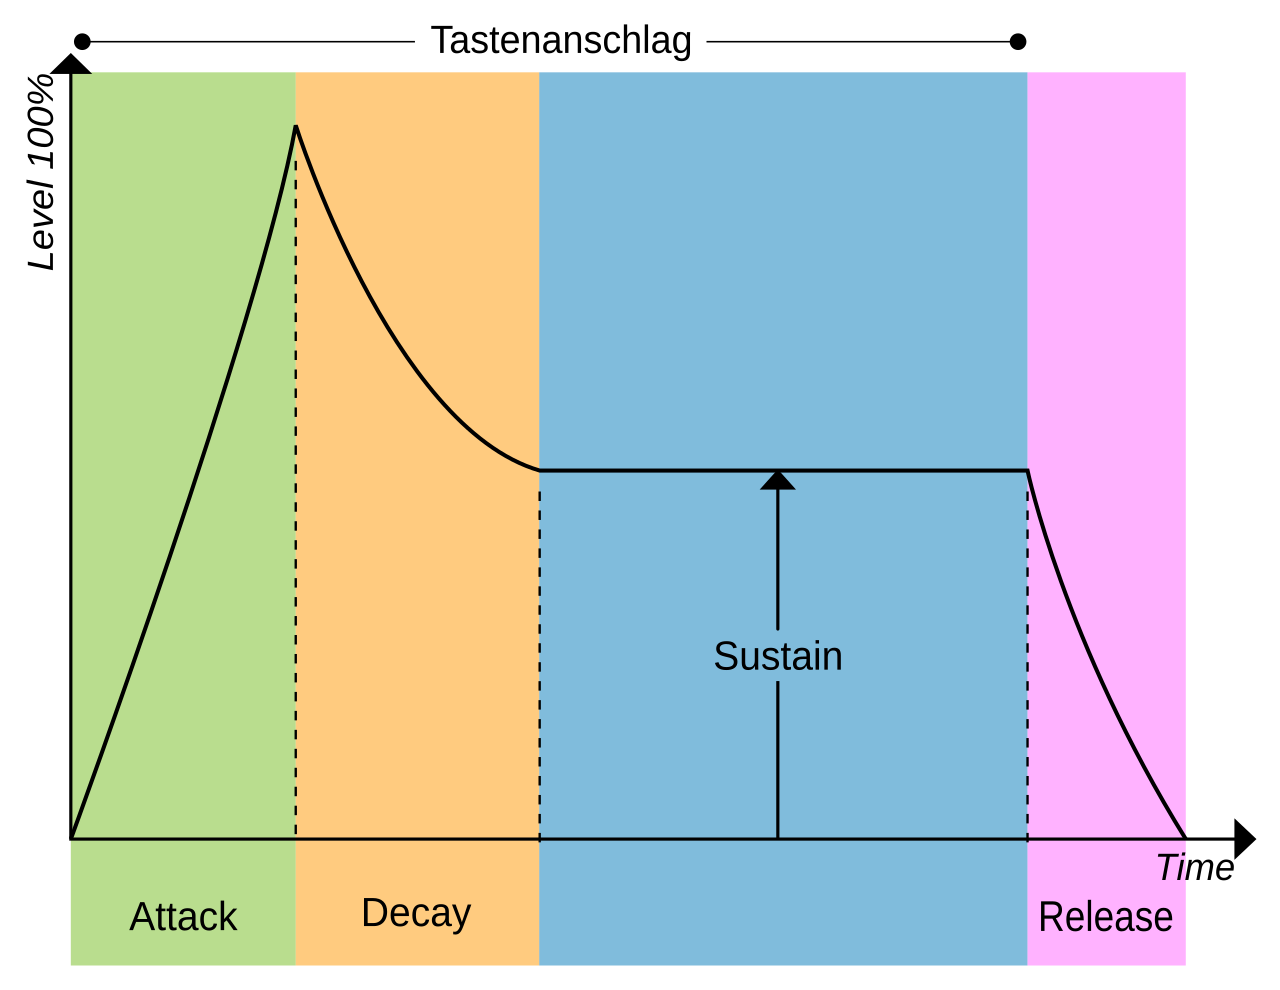
\includegraphics[width=0.8\textwidth]{fig/fig_2_5.png}
    \caption{Schematyczna wizualizacja obwiedni dźwięku ADSR (oś pionowa: amplituda, oś pozioma: czas)~\autocite{wiki:adsr}.}
    \label{fig:adsr}
\end{figure}

\subsection{Reprezentacja sygnału audio w dziedzinie czasu i częstotliwości}
\label{ssec:reprezentacja_czas_czestotliwosc}

Cyfrowy sygnał audio jest sekwencją próbek reprezentujących amplitudę fali akustycznej w~kolejnych, dyskretnych punktach czasu~\autocite{KlapuriDavy2006SignalProcessing}. Analiza wyłącznie w~dziedzinie czasu nie ujawnia jednak w~pełni struktury muzycznej sygnału. Kluczowa jest analiza częstotliwościowa, pozwalająca zidentyfikować składowe częstotliwościowe. Przejście z~dziedziny czasu do dziedziny częstotliwości realizowane jest za pomocą transformaty Fouriera, która dekomponuje sygnał na sumę składowych sinusoidalnych o~różnych częstotliwościach i~amplitudach, tworząc jego widmo częstotliwościowe~\autocite{KlapuriDavy2006SignalProcessing}. Dyskretna transformata Fouriera (DFT) jest podstawowym narzędziem tej analizy. Dla skończonego ciągu próbek sygnału~$x_n$ o~długości~N, jej k-ty współczynnik~$X_k$ jest zdefiniowany wzorem~(\ref{eq:dft}):
\begin{equation}
    X_k = \sum_{n=0}^{N-1} x_n \cdot e^{-i\frac{2\pi}{N}kn}
    \label{eq:dft}
\end{equation}
gdzie $n$ jest indeksem próbki w~dziedzinie czasu, $k$ jest indeksem częstotliwości, a~$i$ jest jednostką urojoną. Działanie transformaty ilustruje rysunek~\ref{fig:fig_2_1}.

\begin{figure}[!htbp]
    \centering
    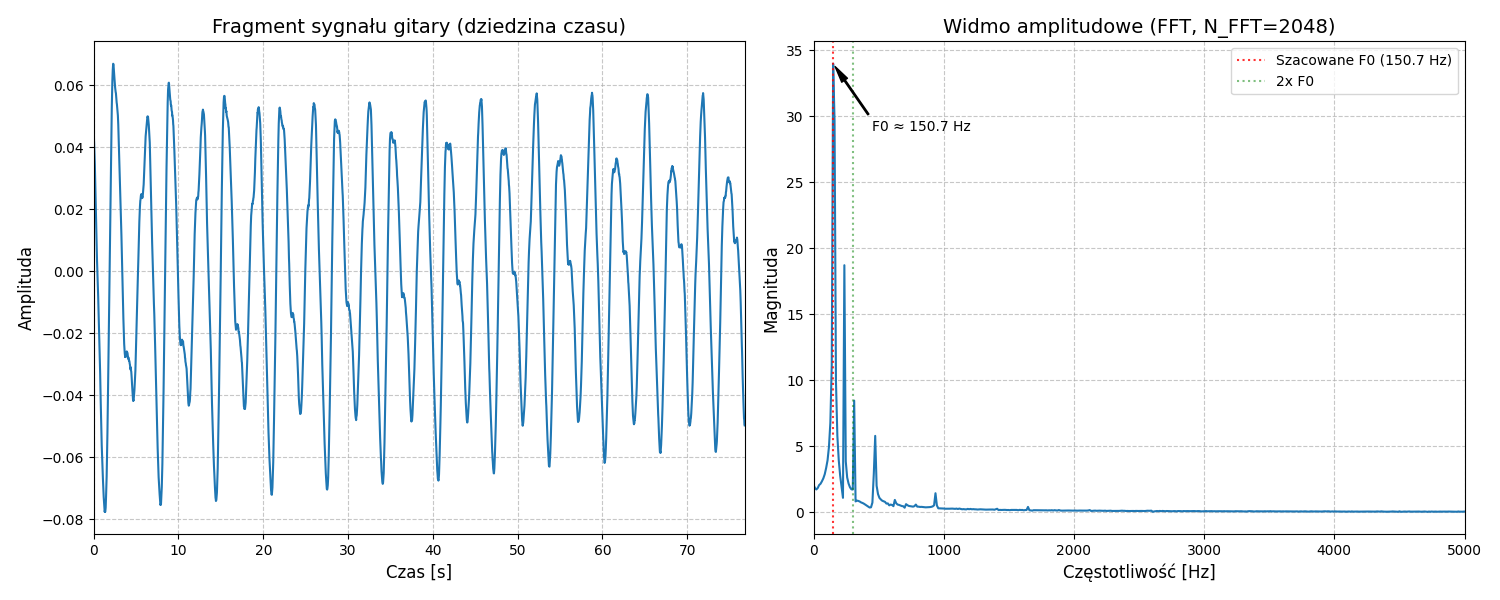
\includegraphics[width=\textwidth]{fig/fig_2_1.png}
    \caption{Po lewej: fragment sygnału audio pojedynczego dźwięku gitary w~dziedzinie czasu (oś pionowa: amplituda (wartość znormalizowana), oś pozioma: czas w~próbkach). Po prawej: odpowiadające mu widmo amplitudowe (oś pionowa: magnituda (jednostki względne), oś pozioma: częstotliwość w~Hz), ukazujące częstotliwość podstawową ($F_0$) oraz jej kolejne alikwoty (składowe harmoniczne).}
    \label{fig:fig_2_1}
\end{figure}

\subsection{Analiza czasowo-częstotliwościowa i jej znaczenie dla ATM}
\label{ssec:analiza_czas_czestotliwosc}

Charakterystyki częstotliwościowe muzyki zmieniają się w~czasie, dlatego w~zastosowaniach ATM niezbędne są metody analizy czasowo-częstotliwościowej. Podstawową techniką jest krótkoczasowa transformata Fouriera (ang. \textit{Short-Time Fourier Transform}, STFT), która polega na sekwencyjnej analizie Fouriera krótkich, najczęściej nakładających się na siebie segmentów sygnału~\autocite{KlapuriDavy2006SignalProcessing,BurletHindle2017IsolatedGuitarTranscription}. Wynikiem STFT jest spektrogram – dwuwymiarowa reprezentacja energii sygnału w~funkcji czasu i~częstotliwości, która stanowi podstawę dla wielu systemów ATM. Należy pamiętać o~nieodłącznym kompromisie STFT między rozdzielczością czasową a~częstotliwościową, wynikającym z~zasady nieoznaczoności. Kluczowym ograniczeniem tej metody w~kontekście muzycznym jest jej stała rozdzielczość częstotliwościowa, co oznacza, że pasma częstotliwości mają identyczną szerokość (np. w~hercach) na całej skali. Nie odpowiada to logarytmicznej naturze ludzkiej percepcji wysokości dźwięku.

\begingroup
\sloppy
W odpowiedzi na to ograniczenie opracowano alternatywne reprezentacje, lepiej dostosowane do specyfiki sygnału muzycznego. Jedną z~nich jest transformata Constant-Q (ang. \textit{Constant-Q Transform}, CQT)~\autocite{Benetos2019AutomaticMusicTranscription,Wiggins2019TabCNN,Zang2023SynthTab}. Jej fundamentalną cechą jest zastosowanie logarytmicznej skali częstotliwości, która naśladuje strukturę skal muzycznych. W~praktyce, CQT dzieli oś częstotliwości na pasma (tzw. prążki), których szerokości są geometrycznie rozmieszczone, co skutkuje stałą liczbą pasm na oktawę. Taka organizacja zapewnia zmienną rozdzielczość: wysoką w~dziedzinie częstotliwości dla niskich tonów, co ułatwia rozróżnianie nut podstawowych, oraz wysoką w~dziedzinie czasu dla tonów wysokich, co jest korzystne dla analizy szybkich transjentów i~alikwotów.
\endgroup

Inną powszechnie stosowaną nieliniową skalą częstotliwości jest skala Mel, której geneza również leży w~badaniach psychoakustycznych nad ludzką percepcją~\autocite{Benetos2019AutomaticMusicTranscription}. Skala ta nie jest czysto logarytmiczna; jej charakterystyka jest zbliżona do liniowej dla częstotliwości poniżej 1~kHz, a~dopiero powyżej tej granicy staje się coraz bardziej logarytmiczna, odzwierciedlając mniejszą wrażliwość ludzkiego ucha na zmiany wysokości dla wyższych dźwięków. Mel-spektrogramy, czyli spektrogramy z~osią częstotliwości przekształconą na skalę Mel, tworzy się poprzez przetworzenie standardowego spektrogramu STFT za pomocą banku nakładających się na siebie filtrów trójkątnych, których rozmieszczenie odpowiada skali Mel. Proces ten prowadzi do redukcji wymiarowości przy jednoczesnym zachowaniu informacji kluczowych z~punktu widzenia percepcji, co czyni mel-spektrogramy standardowym wejściem dla wielu modeli głębokiego uczenia.

Ewolucja od STFT, poprzez CQT, do mel-spektrogramów odzwierciedla dążenie do tworzenia reprezentacji cech bardziej zgodnych z~ludzką percepcją i~efektywniejszych dla algorytmów uczenia maszynowego. Różne reprezentacje czasowo-częstotliwościowe dla tego samego fragmentu muzycznego wizualizuje rysunek~\ref{fig:fig_2_2}.

\begin{figure}[H]
    \centering
    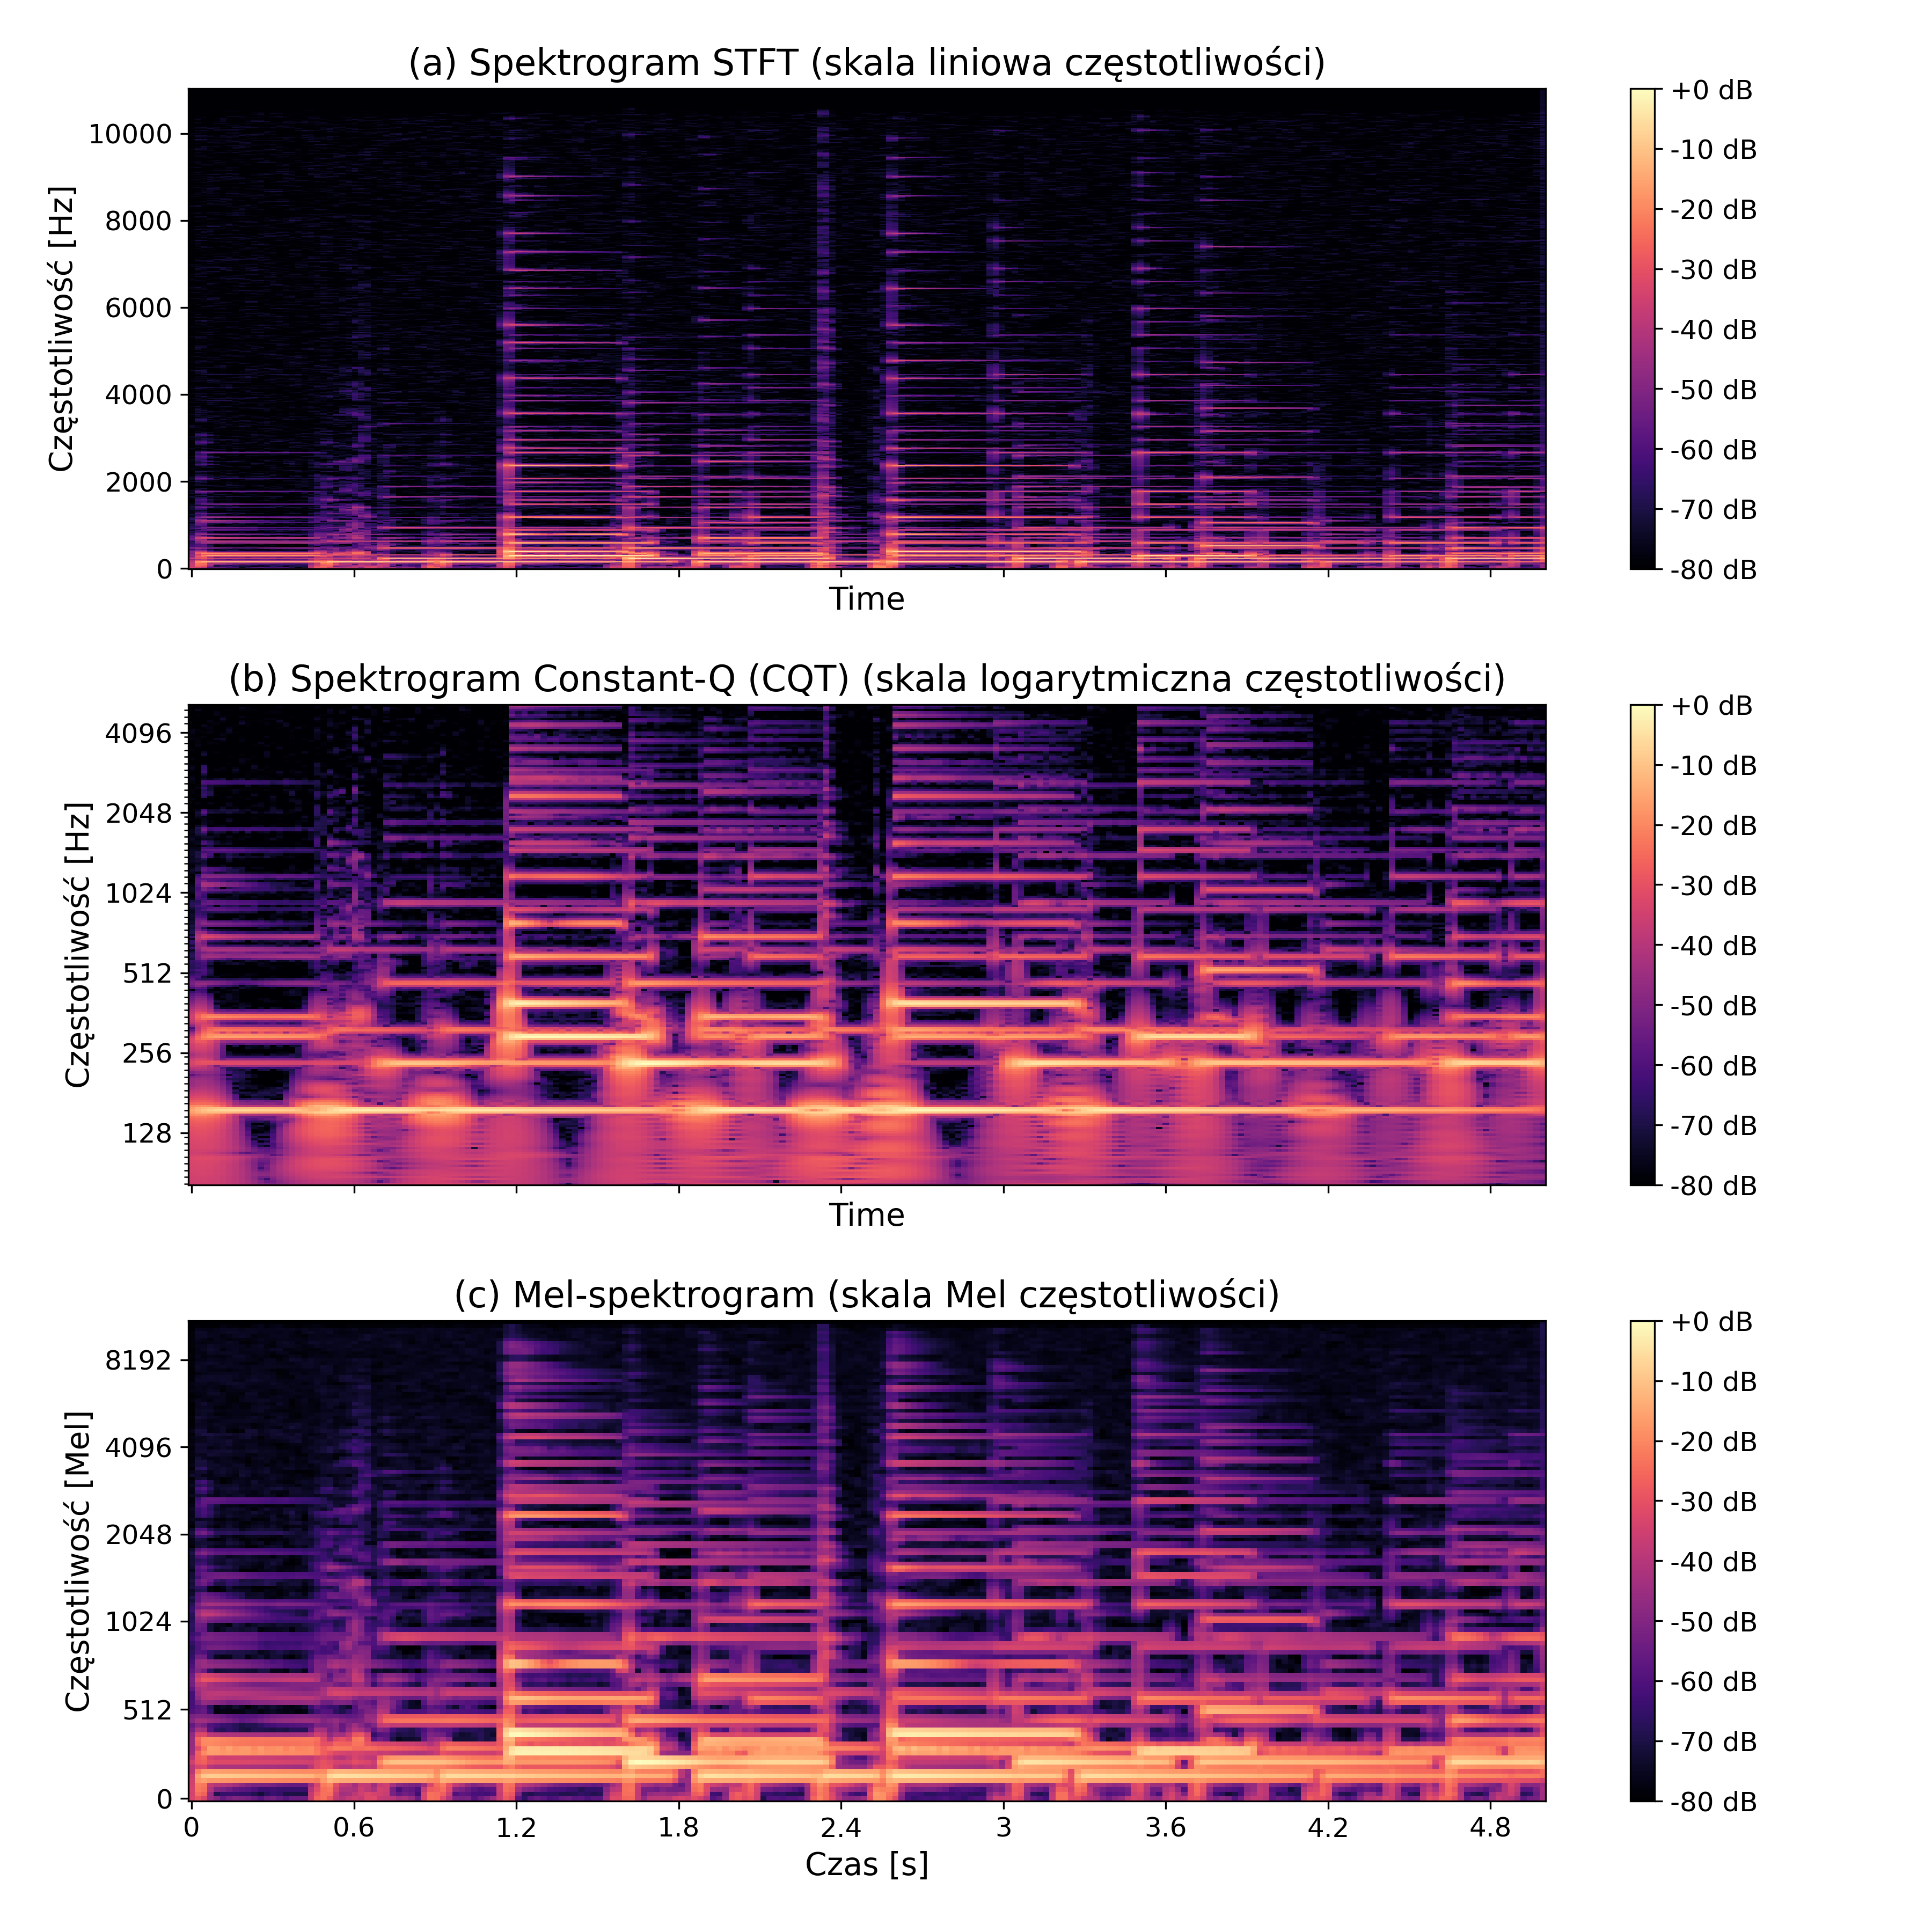
\includegraphics[width=0.85\textwidth]{fig/fig_2_2.png}
    \caption{Wizualizacja różnych reprezentacji czasowo-częstotliwościowych dla tego samego polifonicznego fragmentu gitarowego: (a) Spektrogram STFT z~liniową skalą częstotliwości, (b) Spektrogram Constant-Q (CQT) z~logarytmiczną skalą częstotliwości, (c) Mel-spektrogram z~osią częstotliwości w~skali Mel.}
    \label{fig:fig_2_2}
\end{figure}

\section{Automatyczna transkrypcja muzyczna: zadania, poziomy i wyzwania}
\label{sec:rdzen_atm}

ATM, jest procesem wieloetapowym, obejmującym szereg skomplikowanych zadań cząstkowych. Zrozumienie tych zadań, poziomów abstrakcji, na jakich operują, oraz nieodłącznych wyzwań jest kluczowe dla oceny istniejących rozwiązań i~projektowania nowych.

\subsection{Definicja, zadania składowe i poziomy abstrakcji w ATM}
\label{ssec:definicja_zadania_poziomy_atm}

Formalnie, ATM można zdefiniować jako proces estymacji parametrów nut, takich jak czas rozpoczęcia, wysokość i~czas trwania, bezpośrednio z~sygnału audio~\autocite{KlapuriDavy2006SignalProcessing,Benetos2019AutomaticMusicTranscription}. Jest to zadanie hierarchiczne, które można zdekomponować na kilka kluczowych zadań składowych. Do najważniejszych z~nich należą~\autocite{Benetos2019AutomaticMusicTranscription,Hawthorne2018Onsets}:
\begin{itemize}
    \item \textbf{estymacja wielokrotnej wysokości dźwięku} (ang. \textit{Multiple Pitch Estimation}, MPE), czyli identyfikacja wszystkich częstotliwości podstawowych obecnych w~danym momencie;
    \item \textbf{detekcja początku i~końca dźwięku} (ang. \textit{Onset/Offset Detection}), czyli precyzyjne lokalizowanie w~czasie momentów rozpoczęcia i~zakończenia poszczególnych zdarzeń muzycznych;
    \item \textbf{zadania zaawansowane}, takie jak rozpoznawanie instrumentów, analiza rytmu i~metrum czy interpretacja ekspresji wykonawczej.
\end{itemize}

Wyniki transkrypcji mogą być prezentowane na różnych poziomach abstrakcji~\autocite{Benetos2019AutomaticMusicTranscription}:
\begin{itemize}
    \item \textbf{na poziomie krótkich ramek czasowych}, np. poprzez wskazanie aktywnych wysokości dźwięku w~oknie kilkudziesięciu milisekund;
    \item \textbf{na poziomie symbolicznym}, jako zestaw nut z~określonymi atrybutami;
    \item \textbf{na poziomie strukturalnym}, jako bardziej złożone obiekty, takie jak strumienie melodyczne czy pełna partytura muzyczna.
\end{itemize}

\begin{figure}[!htbp]
    \centering
    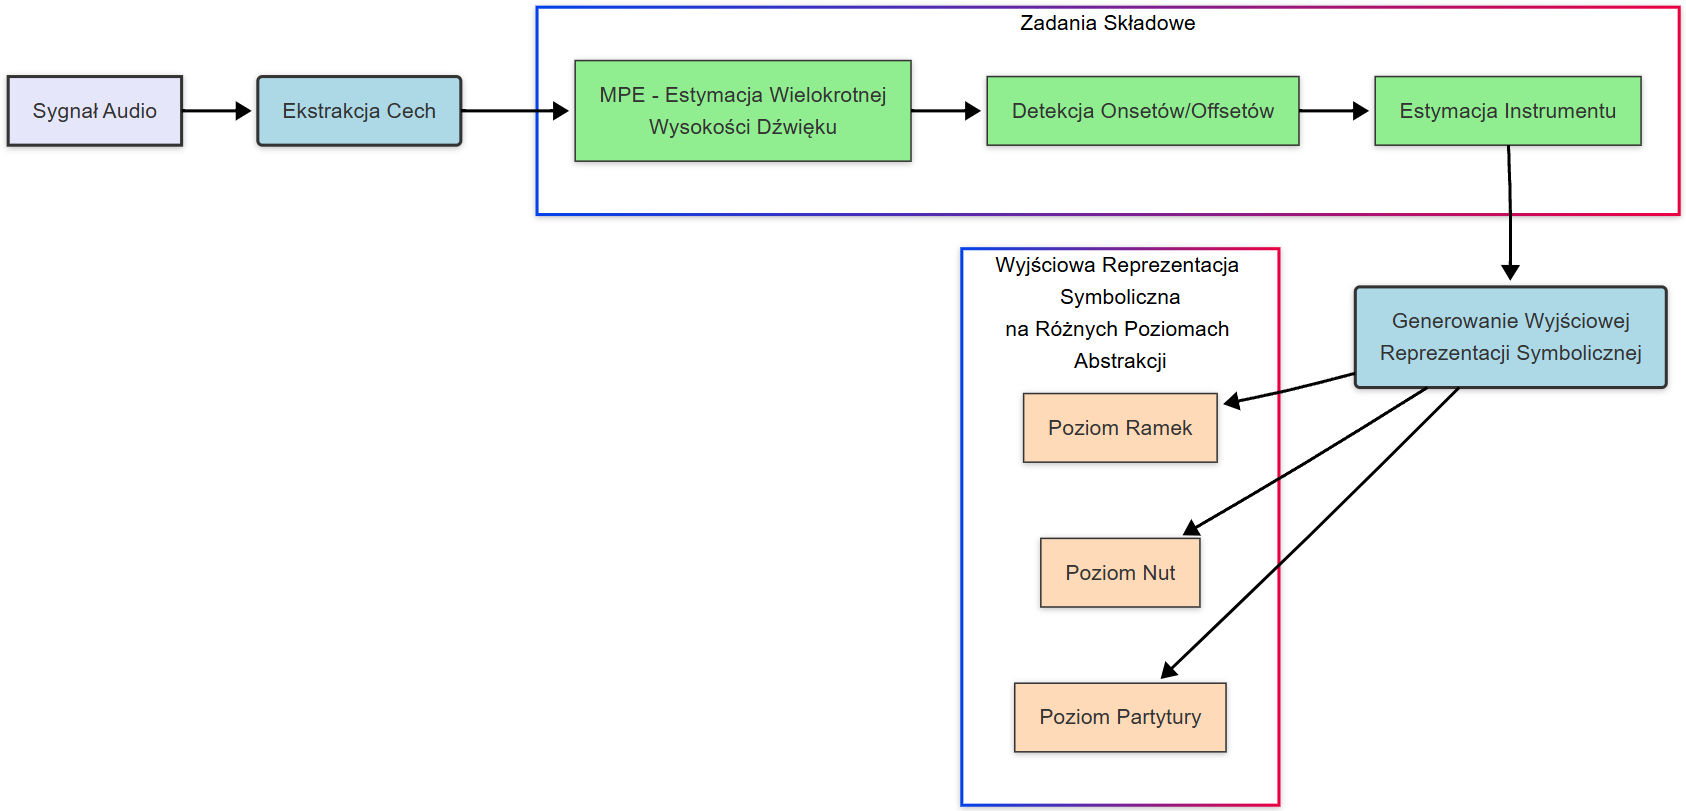
\includegraphics[width=1.0\textwidth]{fig/fig_2_3.png}
    \caption{Uproszczony schemat potoku przetwarzania w~systemie ATM: od sygnału audio, poprzez ekstrakcję cech, zadania składowe (MPE, detekcja onsetów/offsetów, estymacja instrumentu), aż po generowanie wyjściowej reprezentacji symbolicznej na różnych poziomach abstrakcji (ramki, nuty, partytura)~\autocite{Benetos2019AutomaticMusicTranscription}.}
    \label{fig:fig_2_3}
\end{figure}

\subsection{Transkrypcja monofoniczna vs polifoniczna – złożoność i główne wyzwania}
\label{ssec:mono_vs_poli_wyzwania}

Złożoność zadania ATM znacząco wzrasta przy przejściu od transkrypcji monofonicznej (pojedyncza linia melodyczna) do polifonicznej (wiele współbrzmiących dźwięków)~\autocite{KlapuriDavy2006SignalProcessing,Benetos2019AutomaticMusicTranscription}. Muzyka gitarowa, ze względu na możliwość gry akordowej i~prowadzenia wielu niezależnych linii melodycznych, jest w~przeważającej mierze polifoniczna, co czyni jej transkrypcję szczególnie trudną~\autocite{BurletHindle2017IsolatedGuitarTranscription}. Główne wyzwania w~ATM, które ulegają intensyfikacji w~kontekście polifonii, to przede wszystkim: interferencja harmonicznych składowych różnych dźwięków (szczególnie w~interwałach konsonansowych), maskowanie cichszych dźwięków przez głośniejsze, trudności w~precyzyjnej detekcji czasów rozpoczęcia i~zakończenia dźwięków w~gęstych fakturach, zmienność barwy dźwięku zależna od artykulacji i~dynamiki, oraz częste błędy w~estymacji wysokości, takie jak pomyłki oktawowe~\autocite{Benetos2019AutomaticMusicTranscription}. Dodatkowo, efektywne trenowanie modeli uczenia maszynowego wymaga dostępu do dużych, dokładnie zaanotowanych zbiorów danych, których tworzenie jest procesem czasochłonnym i~kosztownym.
%Początek
\section{Przegląd metod stosowanych w automatycznej transkrypcji muzycznej}
\label{sec:przeglad_metod_atm}

Rozwój metod ATM jest procesem ciągłym, odzwierciedlającym postęp w~dziedzinach przetwarzania sygnałów i~uczenia maszynowego. Poniżej przedstawiono ewolucję tych podejść, od metod klasycznych po najnowsze techniki oparte na głębokim uczeniu.

\subsection{Metody tradycyjne oparte na przetwarzaniu sygnałów}
\label{ssec:tradycyjne_metody_cps}

Historycznie pierwsze podejścia do ATM opierały się w~dużej mierze na technikach CPS~\autocite{KlapuriDavy2006SignalProcessing}. W~przypadku transkrypcji muzyki monofonicznej, gdzie w~danym momencie występuje tylko jeden dźwięk, opracowano szereg metod detekcji jego częstotliwości podstawowej ($F_0$). Do klasycznych algorytmów należą te bazujące na analizie funkcji autokorelacji (ang. \textit{Auto-Correlation Function}, ACF), uśrednionej funkcji różnicowej amplitudy (ang. \textit{Average Magnitude Difference Function}, AMDF), technice spektrum harmonicznego iloczynu (ang. \textit{Harmonic Product Spectrum}, HPS), która wzmacnia częstotliwość podstawową poprzez mnożenie widma z~jego wersjami skompresowanymi w~dziedzinie częstotliwości (tj. widmami poddanymi decymacji), oraz na analizie cepstralnej (ang. \textit{cepstral analysis}). Cepstrum, będące wynikiem odwrotnej transformaty Fouriera z~logarytmu widma mocy sygnału, pozwala na separację składowej związanej ze źródłem dźwięku (pobudzeniem) od składowej związanej z~charakterystyką filtru rezonansowego instrumentu~\autocite{KlapuriDavy2006SignalProcessing}. Rozwijano również systemy bazujące na modelach harmonicznych dźwięku oraz systemy ekspertowe, wykorzystujące predefiniowane reguły i~wiedzę muzykologiczną~\autocite{KlapuriDavy2006SignalProcessing}. Metody te wykazywały znaczne ograniczenia w~kontekście analizy muzyki polifonicznej, gdzie jednoczesne występowanie wielu dźwięków i~ich alikwotów znacząco komplikuje sygnał, prowadząc m.in. do niemożności separacji nakładających się szeregów harmonicznych. Ograniczenia te stały się motywacją do poszukiwania bardziej zaawansowanych rozwiązań w~ramach uczenia maszynowego.

\subsection{Metody oparte na uczeniu maszynowym}
\label{ssec:metody_uczenia_maszynowego_atm}

Przełom w~skuteczności systemów ATM przyniosło zastosowanie metod uczenia maszynowego, które pozwoliły na tworzenie modeli zdolnych do nauki złożonych zależności bezpośrednio z~danych~\autocite{Jamshidi2024SurveyAMT,BurletHindle2017IsolatedGuitarTranscription}. W~ramach tego paradygmatu można wyróżnić kilka głównych kierunków.

\subsubsection{Nienadzorowane metody faktoryzacji macierzy}
\label{sssec:nmf_atm}

Wśród metod nienadzorowanych, popularność zdobyła nieujemna faktoryzacja macierzy (ang. \textit{Non-negative Matrix Factorization}, NMF)~\autocite{Benetos2019AutomaticMusicTranscription}. W kontekście muzycznym, technika ta polega na dekompozycji (rozłożeniu) macierzy wejściowej, którą jest spektrogram, na iloczyn dwóch macierzy o mniejszych wymiarach, również posiadających wyłącznie wartości nieujemne.

Pierwsza z nich, \textbf{macierz szablonów} (słownika), zawiera zbiór charakterystycznych profili spektralnych. Każdy taki profil można interpretować jako ``dźwiękowy odcisk palca'' pojedynczej nuty, ukazujący rozkład energii na jej częstotliwość podstawową i kolejne harmoniczne. Druga macierz, \textbf{macierz aktywacji}, określa z kolei, z jaką głośnością i w którym momencie każdy z tych szablonów pojawia się w oryginalnym nagraniu. W ten sposób spektrogram całego utworu jest reprezentowany jako suma ważona podstawowych komponentów muzycznych.

Zaletą NMF jest jej zdolność do automatycznego, nienadzorowanego odkrywania tych fundamentalnych struktur w danych. Istotnym wyzwaniem jest jednak fakt, że podstawowa wersja NMF może mieć trudności z separacją źródeł o silnie nakładających się charakterystykach spektralnych -- na przykład dźwięków w konsonansowych interwałach, których harmoniczne pokrywają się. W celu rozwiązania tych problemów opracowano liczne rozszerzenia NMF, takie jak nadzorowane NMF (gdzie szablony są predefiniowane i stałe) czy harmoniczne NMF (które narzucają harmoniczną strukturę na szablony, zapewniając ich muzyczną poprawność)~\autocite{Benetos2019AutomaticMusicTranscription}.

\subsubsection{Modele probabilistyczne i bayesowskie}
\label{sssec:modele_probabilistyczne_atm}

Ukryte modele Markowa (ang. \textit{Hidden Markov Models}, HMM) były przez wiele lat intensywnie badane i~stosowane w~ATM, głównie ze względu na ich naturalną zdolność do modelowania sekwencyjnego charakteru muzyki~\autocite{KlapuriDavy2006SignalProcessing,Cazau2017HMM,Raphael2002PianoTranscription}. W~typowym podejściu, ukryte stany HMM mogą odpowiadać poszczególnym nutom lub stanom ciszy, a~obserwacje emitowane przez te stany to wektory cech akustycznych wyekstrahowanych z~kolejnych ramek sygnału audio. Prace Raphaela~\autocite{Raphael2002PianoTranscription} stanowią wczesny przykład zastosowania HMM do transkrypcji muzyki fortepianowej, gdzie modelowano proces generowania nut z~uwzględnieniem prawdopodobieństw przejść między nimi. Cazau i~Nuel~\autocite{Cazau2017HMM} eksplorowali różne warianty HMM, w~tym ich integrację z~metodami dekompozycji spektralnej, jak probabilistyczna analiza składowych ukrytych (ang. \textit{Probabilistic Latent Component Analysis}, PLCA), w~celu poprawy jakości transkrypcji, np. poprzez modelowanie trwania nut lub wykorzystanie wiedzy o~tonalności do modelowania przejść harmonicznych. Podejścia bayesowskie, stanowiące szerszą klasę modeli, pozwalają na formalne włączenie do modelu wcześniejszej wiedzy (np. reguł harmonii, typowych progresji akordów) w~postaci rozkładów a~priori. Mimo pewnych sukcesów, modele te często wymagają starannej inżynierii cech i~mogą mieć trudności z~modelowaniem bardzo złożonych zależności w~muzyce polifonicznej.

\subsubsection{Głębokie sieci neuronowe}
\label{sssec:deep_learning_atm}

W ostatnich latach metody oparte na głębokim uczeniu (DL) zdominowały badania nad ATM, osiągając wyniki stanowiące aktualny stan wiedzy w~wielu aspektach tego zadania~\autocite{Benetos2019AutomaticMusicTranscription,Jamshidi2024SurveyAMT}. Zdolność głębokich sieci neuronowych do automatycznego uczenia się hierarchicznych, wielopoziomowych reprezentacji cech bezpośrednio z~danych wejściowych (np. surowych spektrogramów) okazała się kluczowa dla postępu. Wśród najczęściej wykorzystywanych architektur znajdują się konwolucyjne sieci neuronowe (ang. \textit{Convolutional Neural Networks}, CNN), efektywnie przetwarzające dane o~strukturze siatki, takie jak spektrogramy~\autocite{Wiggins2019TabCNN,Zang2023SynthTab}; rekurencyjne sieci neuronowe (ang. \textit{Recurrent Neural Networks}, RNN), w~szczególności warianty z~długą krótkotrwałą pamięcią (ang. \textit{Long Short-Term Memory}, LSTM) i~bramkowanymi jednostkami rekurencyjnymi (ang. \textit{Gated Recurrent Unit}, GRU), przystosowane do modelowania zależności czasowych w~sekwencjach muzycznych~\autocite{Benetos2019AutomaticMusicTranscription}; oraz architektury hybrydowe, takie jak konwolucyjno-rekurencyjne sieci neuronowe (ang. \textit{Convolutional Recurrent Neural Network}, CRNN), łączące zalety obu tych podejść~\autocite{Hawthorne2018Onsets}. Najnowsze badania eksplorują również potencjał architektur opartych na mechanizmach uwagi, takich jak Transformer (ang. \textit{Transformer})~\autocite{Jamshidi2024SurveyAMT,Hawthorne2021Seq2SeqTranscription}.
Dostępność dużych, publicznych zbiorów danych adnotowanych, takich jak MAESTRO dla muzyki fortepianowej~\autocite{Hawthorne2018Onsets,Zang2023SynthTab} (zawierający nagrania z~konkursów pianistycznych wraz z~odpowiadającymi im plikami MIDI) oraz GuitarSet dla muzyki gitarowej~\autocite{Wiggins2019TabCNN,Zang2023SynthTab,Benetos2019AutomaticMusicTranscription} (oferujący nagrania z~sześciu osobnych przetworników dla każdej struny oraz zsynchronizowane adnotacje MIDI i~tabulaturowe), była katalizatorem rozwoju modeli DL. To właśnie te obszerne i~zaanotowane zbiory danych umożliwiły trenowanie złożonych modeli DL na skalę niezbędną do osiągnięcia wysokiej dokładności, podkreślając, że postęp w~tej dziedzinie jest równie mocno zależny od inżynierii danych, co od innowacji algorytmicznych. Model ,,Onsets and Frames''~\autocite{Hawthorne2018Onsets}, zaprojektowany do transkrypcji muzyki fortepianowej, jest przykładem systemu DL, który osiągnął wysoką skuteczność. Wykorzystuje on architekturę CRNN do jednoczesnej predykcji czasów rozpoczęcia dźwięków (ang. \textit{onsets}) oraz aktywności poszczególnych nut w~kolejnych ramkach czasowych. ,,Basic Pitch''~\autocite{Bittner2022BasicPitch} to z~kolei narzędzie typu audio-to-MIDI, opracowane przez Spotify, które charakteryzuje się lekkością i~zdolnością do detekcji zmian wysokości dźwięku (ang. \textit{pitch bends}). Opiera się na modelach CNN, a~jego priorytetem jest szybkość działania i~dostępność, co czyni je użytecznym w~wielu praktycznych zastosowaniach, chociaż może nie osiągać takiej samej szczegółowości transkrypcji jak bardziej złożone systemy w~przypadku skomplikowanych fragmentów polifonicznych. Mimo imponujących wyników, metody DL nie są pozbawione ograniczeń. Ich skuteczność jest silnie uzależniona od ilości i~jakości danych treningowych, a~trening i~inferencja złożonych modeli DL mogą być wymagające obliczeniowo~\autocite{Jamshidi2024SurveyAMT}.

%Koniec
\section{Specyfika transkrypcji muzyki gitarowej na zapis tabulaturowy (GTT)}
\label{sec:specyfika_gtt}

Transkrypcja muzyki gitarowej, zwłaszcza z~celem wygenerowania zapisu tabulaturowego, wprowadza szereg specyficznych problemów i~wymagań, które odróżniają ją od ogólnego zadania ATM. Niniejsza sekcja poświęcona jest analizie tych unikalnych aspektów.

\subsection{Akustyczna charakterystyka sygnału gitary i jej implikacje dla transkrypcji}
\label{ssec:akustyka_gitary_gtt}

Sygnał generowany przez gitarę posiada szereg unikalnych cech akustycznych, które czynią jego automatyczną transkrypcję zadaniem szczególnie złożonym~\autocite{Wiggins2019TabCNN,BurletHindle2017IsolatedGuitarTranscription}. Obwiednia dźwięku gitary, zwłaszcza akustycznej, charakteryzuje się zazwyczaj bardzo szybkim atakiem i~relatywnie długim, stopniowym wybrzmiewaniem, co może utrudniać precyzyjną detekcję czasów zakończenia dźwięków (ang. \textit{offsets}). Barwa dźwięku gitary jest niezwykle zróżnicowana i~zależy od wielu czynników, takich jak konstrukcja instrumentu (np. gitara akustyczna z~pudłem rezonansowym, gitara elektryczna typu \textit{solid-body}), rodzaj i~wiek strun, technika artykulacji (np. gra kostką, palcami, techniką \textit{slap}), a~w~przypadku gitar elektrycznych~– w~decydującym stopniu od ustawień wzmacniacza oraz zastosowanych efektów gitarowych (np. \textit{distortion, overdrive, chorus, flanger, delay, reverb})~\autocite{Wiggins2019TabCNN}. Ta nieodłączna zmienność i~bogactwo barwowe, choć stanowią o~atrakcyjności instrumentu, komplikują proces tworzenia uogólnionych modeli transkrypcyjnych. Kluczowe dla GTT jest również adekwatne uwzględnienie licznych, specyficznych dla gitary technik wykonawczych, których manifestacje akustyczne przedstawia Tabela~\ref{tab:techniki_gitarowe_latex_poprawiona}. Techniki te nie tylko znacząco wpływają na charakterystykę sygnału, ale także mają swoje bezpośrednie odzwierciedlenie w~zapisie tabulaturowym.

\begin{longtable}{|p{0.18\textwidth}|p{0.39\textwidth}|p{0.33\textwidth}|}
    \caption[Wybrane techniki gitarowe i ich manifestacje akustyczne]{Akustyczne manifestacje wybranych technik gitarowych istotnych dla transkrypcji na tabulaturę.}
    \label{tab:techniki_gitarowe_latex_poprawiona} \\
    \hline
    \textbf{Technika} & \textbf{Opis} & \textbf{Akustyczna Manifestacja (Przykładowa)} \\
    \hline
    \endfirsthead
    \hline
    \textbf{Technika} & \textbf{Opis} & \textbf{Akustyczna Manifestacja (Przykładowa)} \\
    \hline
    \endhead
    \hline
    \endfoot
    \hline
    \endlastfoot
    (ang. \textit{Hammer-on}) & Uderzenie palcem lewej ręki (dla praworęcznych gitarzystów) w~strunę na wyższym progu w~celu wydobycia dźwięku bez ponownego szarpania struny prawą ręką.
    & Zazwyczaj łagodniejszy atak spektralny w~porównaniu do dźwięku szarpniętego; możliwy spadek amplitudy po wykonaniu techniki, szczególnie na cieńszych strunach~\autocite{Nasution2023HammerOn};
    poprzedzający dźwięk (jeśli był) może wybrzmiewać w~tle z~niższą amplitudą~\autocite{Nasution2023HammerOn,Su2014SparseCepstral}.
    Brak wyraźnego ,,dołka'' w~amplitudzie między nutami w~sekwencji legato~\autocite{Reboursiere2011GuitarController}.
    \\
    \hline
    (ang. \textit{Pull-off}) & Oderwanie palca lewej ręki od struny (zazwyczaj z~lekkim jej szarpnięciem) w~celu wydobycia niższego dźwięku, który już brzmi (np. na pustej strunie lub przytrzymywany innym palcem na niższym progu).
    & Podobnie jak \textit{hammer-on}, charakteryzuje się łagodniejszym atakiem w~porównaniu do dźwięku szarpniętego; zmiana wysokości następuje na niższą;
    może towarzyszyć krótki, szerokopasmowy szum związany z~mechanicznym ruchem odrywania palca~\autocite{Su2014SparseCepstral}.
    \\
    \hline
    (ang. \textit{Slide}) (ślizg) & Płynne przesunięcie palca lewej ręki wzdłuż struny pomiędzy dwoma progami, podczas gdy struna wibruje.
    & Ciągła, płynna zmiana częstotliwości podstawowej ($F_0$) i~jej harmonicznych (tzw. \textit{glissando}) między wysokością początkową a~końcową~\autocite{Su2014SparseCepstral,Reboursiere2011GuitarController};
    zachowanie energii sygnału i~jego ciągłości spektralnej; charakterystyczny profil przejścia między wysokościami, odróżniający od techniki \textit{bend}~\autocite{Su2014SparseCepstral}.
    \\
    \hline
    (ang. \textit{Bend}) (podciągnięcie) & Poprzeczne podciągnięcie struny na gryfie palcem lewej ręki, co zwiększa jej napięcie i~w~rezultacie podwyższa wysokość dźwięku.
    & Płynna zmiana wysokości dźwięku ($F_0$) w~górę, często z~następującym powrotem do oryginalnej wysokości lub przejściem do innej~\autocite{Su2014SparseCepstral,Reboursiere2011GuitarController};
    mogą pojawić się charakterystyczne zmiany w~natężeniu alikwotów oraz subtelne zmiany barwy.
    \\
    \hline
    (ang. \textit{Palm-muting}) & Delikatne tłumienie strun krawędzią dłoni prawej ręki (dla gitarzystów praworęcznych) w~pobliżu mostka gitary, bezpośrednio po ich szarpnięciu.
    & Znaczne skrócenie czasu wybrzmiewania dźwięku (szybszy zanik energii); stłumiony, bardziej perkusyjny i~mniej rezonujący charakter;
    redukcja udziału wyższych harmonicznych w~spektrum, co prowadzi do ,,ciemniejszego'', ,,cichszego'' brzmienia~\autocite{Su2014SparseCepstral}.
    \\
    \hline
    (ang. \textit{Vibrato}) & Cykliczna, subtelna modulacja wysokości dźwięku, uzyskiwana przez oscylacyjny ruch palca przytrzymującego strunę na progu lub za pomocą ramienia tremolo.
    & Okresowe, stosunkowo wolne (typowo 5-7 Hz) fluktuacje częstotliwości podstawowej ($F_0$) i~jej harmonicznych wokół centralnej wysokości dźwięku~\autocite{Anand2012Vibrato,HyrkasSmyth2024Vibrato};
    może również występować sprzężona z~tym modulacja amplitudy~\autocite{Anand2012Vibrato,HyrkasSmyth2024Vibrato}.
    \\
\end{longtable}

\subsection{Porównanie notacji standardowej i tabulaturowej dla gitary}
\label{ssec:porownanie_notacji_gitara}

W praktyce muzycznej gitarzyści posługują się dwoma głównymi systemami notacji: tradycyjną notacją muzyczną opartą na pięciolinii oraz tabulaturą gitarową. Każdy z~tych systemów posiada swoje unikalne cechy, które determinują jego adekwatność w~różnych zastosowaniach i~dla różnych grup użytkowników~\autocite{Wiggins2019TabCNN}. Tabela~\ref{tab:porownanie_notacji_latex} przedstawia zwięzłe porównanie obu systemów. Wybór tabulatury jako docelowej formy zapisu w~wielu współczesnych systemach GTT jest motywowany jej dużą popularnością, zwłaszcza wśród gitarzystów samouków i~w~muzyce rozrywkowej, oraz jej bezpośrednim, instruktażowym charakterem, który ułatwia naukę i~wykonanie utworu na instrumencie.

\begin{table}[H]
    \centering
    \caption{Porównanie standardowej notacji muzycznej i~tabulatury gitarowej.}
    \label{tab:porownanie_notacji_latex}
    \begin{tabular}{|p{0.2\textwidth}|p{0.38\textwidth}|p{0.32\textwidth}|}
        \hline
        \textbf{Cecha} & \textbf{Standardowa Notacja Muzyczna} & \textbf{Tabulatura Gitarowa} \\
        \hline
        Reprezentacja wysokości & Abstrakcyjna, poprzez pozycję nuty na pięciolinii, wymagająca znajomości klucza i~zasad teorii muzyki~\autocite{Wiggins2019TabCNN}.
        & Bezpośrednia, poprzez wskazanie numeru progu na linii reprezentującej konkretną strunę gitary~\autocite{Wiggins2019TabCNN}.
        \\
        \hline
        Reprezentacja rytmu & Precyzyjnie zdefiniowana za pomocą wartości rytmicznych nut, pauz i~oznaczeń metrycznych~\autocite{Wiggins2019TabCNN}.
        & Często uproszczona lub nieobecna; główny nacisk kładziony jest na wysokość i~sposób opalcowania. Rytm bywa jednak dodawany za pomocą symboli podobnych do notacji standardowej lub poprzez odniesienie do nagrania~\autocite{Wiggins2019TabCNN}.
        \\
        \hline
        Czytelność dla gitarzystów & Wymaga dłuższego procesu nauki i~praktyki w~czytaniu nut na pięciolinii~\autocite{Wiggins2019TabCNN}.
        & Zazwyczaj bardzo intuicyjna i~łatwa do szybkiego opanowania, szczególnie dla początkujących gitarzystów i~samouków; bezpośrednio pokazuje, gdzie umieścić palce na gryfie~\autocite{Wiggins2019TabCNN}. \\
        \hline
        Notacja technik gry & Możliwa za pomocą licznych dodatkowych symboli i~oznaczeń słownych, ale czasami może być mniej jednoznaczna lub intuicyjna dla specyficznych technik gitarowych.
        & Bardzo dobrze przystosowana do notowania szerokiego spektrum specyficznych technik gitarowych (np. \textit{bends, slides, hammer-ons, pull-offs, vibrato}) za pomocą dedykowanych symboli graficznych.
        \\
        \hline
        Niejednoznaczność opalcowania & Istnieje~– ten sam dźwięk (wysokość) może być zagrany na gitarze na kilku różnych strunach i~progach; wybór konkretnego opalcowania jest pozostawiony wykonawcy~\autocite{Wiggins2019TabCNN}. & Zazwyczaj jednoznacznie określa zarówno strunę, jak i~próg, na którym dany dźwięk ma być zagrany, tym samym eliminując problem wyboru opalcowania dla danej nuty~\autocite{Wiggins2019TabCNN}.
        \\
        \hline
    \end{tabular}
\end{table}

\subsection{Kluczowe wyzwania w automatycznej transkrypcji gitary na tabulaturę (GTT)}
\label{ssec:wyzwania_gtt}

Transkrypcja na tabulaturę wprowadza szereg specyficznych wyzwań, które wykraczają poza ogólne problemy ATM:
\begin{itemize}
    \item \textbf{Wysoka polifonia i~nakładanie się dźwięków}: Gitara, jako instrument harmoniczny, często generuje złożone współbrzmienia, co intensyfikuje problem separacji i~identyfikacji poszczególnych dźwięków w~sygnale audio~\autocite{BurletHindle2017IsolatedGuitarTranscription}.
    \item \textbf{Niejednoznaczność reprezentacji dźwięku na gryfie} (ang. \textit{Tablature Inference / Fingering Estimation}): Jest to jedno z~fundamentalnych wyzwań w~GTT. Ten sam dźwięk (o tej samej wysokości muzycznej) może być zagrany w~wielu różnych pozycjach na gryfie gitary (tj. na różnych kombinacjach struny i~progu)~\autocite{Wiggins2019TabCNN}. Wybór konkretnej pozycji przez gitarzystę zależy od wielu czynników, takich jak kontekst muzyczny (np. sąsiednie dźwięki), grywalność (łatwość wykonania danego pochodu dźwięków), preferencje stylistyczne, a~nawet subtelne różnice w~barwie dźwięku uzyskiwane na różnych strunach. System GTT musi więc nie tylko poprawnie zidentyfikować wysokość i~czas trwania nuty, ale również podjąć decyzję co do jej najbardziej prawdopodobnego i/lub optymalnego opalcowania na gryfie. Ilustruje to rysunek~\ref{fig:fig_2_4}.
    \begin{figure}[H]
        \centering
        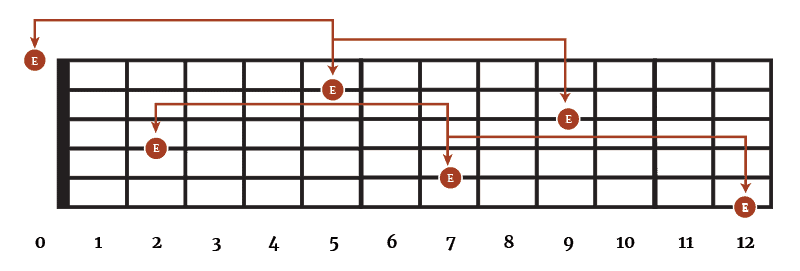
\includegraphics[width=0.6\textwidth]{fig/fig_2_4.png}
        \caption{Przykład tej samej nuty (E4, MIDI 64) możliwej do zagrania w~wielu pozycjach na gryfie gitary standardowo strojonej. Ilustracja przedstawia dźwięk E4 na strunie G (9.~próg), strunie B (5.~próg) oraz pustej strunie wysokiej E. Obrazuje to wyzwanie estymacji opalcowania w~GTT~\autocite{obrazGitaraNiejednoznacznosc}.}
        \label{fig:fig_2_4}
    \end{figure}
    \item \textbf{Zmienność barwy jako potencjalna wskazówka i~problem}: Chociaż subtelne różnice w~barwie dźwięku tej samej nuty granej na różnych strunach mogą teoretycznie dostarczać pewnych wskazówek dla algorytmów estymacji opalcowania, to wszechobecne i~często intensywne stosowanie efektów gitarowych (szczególnie w~muzyce rockowej, metalowej, jazzowej i~elektronicznej) może całkowicie modyfikować oryginalną barwę instrumentu, maskując te subtelne różnice lub wprowadzając własne artefakty, co znacząco komplikuje analizę~\autocite{Wiggins2019TabCNN}.
    \item \textbf{Detekcja i~notacja technik wykonawczych}: Wierne odtworzenie partii gitarowej w~formie tabulatury wymaga nie tylko transkrypcji samych nut, ale również rozpoznania i~odpowiedniego zanotowania licznych, specyficznych dla gitary technik artykulacyjnych (patrz Tabela~\ref{tab:techniki_gitarowe_latex_poprawiona})~\autocite{Reboursiere2011GuitarController,Su2014SparseCepstral}. Jest to zadanie trudne, gdyż akustyczne manifestacje tych technik bywają subtelne i~zmienne.
    \item \textbf{Problem ,,przesunięcia dziedziny''} (ang. \textit{domain shift}): Modele GTT trenowane na danych pochodzących z~jednej domeny (np. czyste, studyjne nagrania gitar akustycznych lub dane syntetyczne) mogą wykazywać znaczący spadek skuteczności, gdy są stosowane do danych z~innej domeny (np. nagrania koncertowe, amatorskie, partie gitar elektrycznych z~efektami)~\autocite{Zang2023SynthTab}. Praca Zang i~współpracowników~\autocite{Zang2023SynthTab} nad zbiorem SynthTab stanowi próbę zaadresowania problemu niedoboru zróżnicowanych danych rzeczywistych poprzez wykorzystanie dużych ilości danych syntetycznych do wstępnego treningu modeli, które następnie mogą być dostrajane na mniejszych zbiorach danych rzeczywistych.
\end{itemize}


\subsection{Przegląd istniejących podejść i narzędzi do GTT}
\label{ssec:podejscia_narzedzia_gtt}

Współczesne podejścia do GTT można generalnie podzielić na dwuetapowe oraz zintegrowane, określane jako (ang. \textit{end-to-end}). Podejścia dwuetapowe realizują zadanie GTT w~dwóch oddzielnych krokach: najpierw dokonuje się ogólnej transkrypcji MPE, a~następnie w~osobnym kroku (inferencji opalcowania) przypisuje się wykryte nuty do pozycji na gryfie~\autocite{BurletHindle2017IsolatedGuitarTranscription}. Zaletą tego podejścia jest jego modularność, a~wadą ryzyko propagacji błędów z~pierwszego etapu.

Podejścia zintegrowane, opierające się w~przeważającej mierze na zaawansowanych modelach DL, dążą do nauczenia się bezpośredniego mapowania z~reprezentacji czasowo-częstotliwościowej na finalną reprezentację tabulaturową. Wykorzystują one złożone architektury sieci neuronowych, takie jak:
\begin{itemize}
    \item Modele oparte na CNN, czego przykładem jest TabCNN~\autocite{Wiggins2019TabCNN}. Architektura ta typowo przetwarza wejściowy spektrogram (np. Constant-Q) i~generuje na wyjściu predykcje dotyczące aktywności poszczególnych progów na każdej ze strun gitary, często w~formacie wielowymiarowej macierzy binarnej (tzw. ,,six-hot encoding''). Praca Zang i~współpracowników~\autocite{Zang2023SynthTab} również wykorzystuje architekturę zbliżoną do TabCNN jako jeden z~modeli bazowych w~swoich badaniach nad wykorzystaniem danych syntetycznych.
    \item Modele oparte na architekturze Transformer, które dzięki zastosowaniu mechanizmów uwagi (ang. \textit{attention mechanisms}) są zdolne do efektywnego modelowania długoterminowych zależności w~danych sekwencyjnych. Znalazły one zastosowanie w~GTT, szczególnie w~połączeniu z~dużymi zbiorami danych, w~tym syntetycznymi, takimi jak SynthTab~\autocite{Zang2023SynthTab}.
    \item Inne architektury, w~tym RNN (np. LSTM czy GRU), często stosowane w~połączeniu z~CNN (tworząc architektury CRNN), aby wykorzystać zdolności CNN do ekstrakcji lokalnych cech ze spektrogramów oraz zdolności RNN do modelowania kontekstu czasowego~\autocite{BurletHindle2017IsolatedGuitarTranscription}. Przykładowo, praca Burlet i~Hindle~\autocite{BurletHindle2017IsolatedGuitarTranscription} badała zastosowanie głębokich sieci przekonań (ang. \textit{Deep Belief Networks}) dla transkrypcji izolowanych dźwięków gitarowych, co stanowiło wczesny przykład wykorzystania metod DL w~tym obszarze.
\end{itemize}
Zaletą podejść zintegrowanych jest ich potencjalna zdolność do uczenia się bardzo złożonych i~subtelnych mapowań bezpośrednio z~danych, co może prowadzić do lepszych wyników końcowych niż w~podejściach dwuetapowych. Wymagają one jednak zazwyczaj znacznie większych i~bardziej szczegółowych zbiorów danych treningowych. Niezależnie od podejścia, kluczową rolę w~rozwoju systemów GTT odgrywają zbiory danych, które zostaną szerzej omówione w~kolejnych rozdziałach.

\section{Podsumowanie i otwarte problemy badawcze}
\label{sec:podsumowanie_analizy_gtt}

Automatyczna transkrypcja muzyczna, a~w~jej ramach transkrypcja muzyki gitarowej na zapis tabulaturowy, pozostaje aktywnym i~wymagającym obszarem badań naukowych. Znaczenie praktyczne skutecznych systemów GTT jest nie do przecenienia, obejmując wsparcie dla muzyków, edukację, archiwizację oraz przemysł muzyczny~\autocite{Benetos2019AutomaticMusicTranscription}. Analiza przeprowadzona w~niniejszym rozdziale wykazała, że główne wyzwania koncentrują się wokół przetwarzania złożonych sygnałów polifonicznych, radzenia sobie z~dużą zmiennością barwy i~artykulacji charakterystyczną dla gitary, a~w~przypadku GTT~– dodatkowo wokół problemu niejednoznaczności opalcowania oraz detekcji i~notacji specyficznych technik wykonawczych~\autocite{Wiggins2019TabCNN}.

Przegląd stosowanych metod ukazuje wyraźną ewolucję od klasycznych technik opartych na przetwarzaniu sygnałów do zaawansowanych modeli uczenia maszynowego, które obecnie definiują stan wiedzy w~tej dziedzinie~\autocite{KlapuriDavy2006SignalProcessing,Jamshidi2024SurveyAMT}. Rozwiązania takie jak ,,Onsets and Frames''~\autocite{Hawthorne2018Onsets} czy ,,Basic Pitch''~\autocite{Bittner2022BasicPitch} dla ogólnych zadań ATM, oraz systemy dedykowane GTT, jak TabCNN~\autocite{Wiggins2019TabCNN} i~nowsze podejścia wykorzystujące duże zbiory danych, w~tym syntetyczne, jak w~przypadku badań nad SynthTab~\autocite{Zang2023SynthTab}, demonstrują znaczący postęp. Mimo to, wciąż istnieją liczne obszary wymagające dalszych, intensywnych badań. Do kluczowych otwartych problemów w~dziedzinie GTT, które wyznaczają kierunki przyszłych prac, należą przede wszystkim:
\begin{enumerate}
    \item Dalsza poprawa dokładności i~odporności transkrypcji w~kontekście gęstych faktur polifonicznych, szybkich pasaży muzycznych oraz sygnałów o~niskiej jakości lub z~silnymi zniekształceniami.
    \item Rozwój bardziej zaawansowanych i~kontekstowych metod inferencji opalcowania na gryfie gitary, które lepiej odzwierciedlałyby rzeczywiste praktyki wykonawcze i~zapewniały grywalność generowanych tabulatur.
    \item Zwiększenie zdolności systemów do rozpoznawania i~poprawnej notacji szerokiego spektrum technik gitarowych, które mają kluczowe znaczenie dla ekspresji muzycznej.
    \item Poprawa generalizacji modeli GTT na różne, nie widziane wcześniej w~procesie treningu, brzmienia gitar (akustycznych, elektrycznych, z~różnymi efektami), style muzyczne i~warunki nagraniowe.
    \item Opracowanie bardziej kompleksowych i~percepcyjnie adekwatnych metryk oceny jakości transkrypcji tabulaturowej, które wykraczałyby poza proste porównanie poprawności nut i~uwzględniałyby aspekty takie jak grywalność, czytelność i~wierność stylistyczną. Kwestia ta nawiązuje do obserwacji, że wyniki ilościowe nie zawsze w~pełni odzwierciedlają praktyczną użyteczność systemu dla końcowego użytkownika~\autocite{Holzapfel2019Ethnomusicology}.
    \item Kontynuacja prac nad tworzeniem i~udostępnianiem większych, bardziej zróżnicowanych i~precyzyjnie adnotowanych zbiorów danych dla GTT, w~tym eksploracja metod efektywnego wykorzystania danych syntetycznych i~technik transferu wiedzy.
\end{enumerate}

Niniejsza praca magisterska stanowi próbę odpowiedzi na niektóre z~wymienionych wyzwań. W~kolejnych rozdziałach przedstawiony zostanie projekt i~implementacja systemu, który w~szczególności skupia się na problemach wyszczególnionych w~punktach (1) i~(2), czyli na poprawie ogólnej dokładności transkrypcji oraz rozwoju metod inferencji opalcowania.  % Analiza tematu
\chapter{[Tytuł rozdziału]} 

%%%%%%%%%%%%%%%%%%%%%
%% RYSUNEK Z PLIKU
%
%\begin{figure}
%\centering
%
\includegraphics[width=0.5\textwidth]{./graf/politechnika_sl_logo_bw_pion_pl.pdf}
%\caption{Podpis rysunku zawsze pod rysunkiem.}
%\label{fig:etykieta-rysunku}
%\end{figure}
%Rys. \ref{fig:etykieta-rysunku} przestawia …
%%%%%%%%%%%%%%%%%%%%%
%
%%%%%%%%%%%%%%%%%%%%%
%% WIELE RYSUNKÓW 
%
%\begin{figure}
%\centering
%\begin{subfigure}{0.4\textwidth}
%    
\includegraphics[width=\textwidth]{./graf/politechnika_sl_logo_bw_pion_pl.pdf}
%    \caption{Lewy górny rysunek.}
%    \label{fig:lewy-gorny}
%\end{subfigure}
%\hfill
%\begin{subfigure}{0.4\textwidth}
%    
\includegraphics[width=\textwidth]{./graf/politechnika_sl_logo_bw_pion_pl.pdf}
%    \caption{Prawy górny rysunek.}
%    \label{fig:prawy-gorny}
%\end{subfigure}
%
%\begin{subfigure}{0.4\textwidth}
%    
\includegraphics[width=\textwidth]{./graf/politechnika_sl_logo_bw_pion_pl.pdf}
%    \caption{Lewy dolny rysunek.}
%    \label{fig:lewy-dolny}
%\end{subfigure}
%\hfill
%\begin{subfigure}{0.4\textwidth}
%    
\includegraphics[width=\textwidth]{./graf/politechnika_sl_logo_bw_pion_pl.pdf}
%    \caption{Prawy dolny rysunek.}
%    \label{fig:prawy-dolny}
%\end{subfigure}
%        
%\caption{Wspólny podpis kilku rysunków.}
%\label{fig:wiele-rysunkow}
%\end{figure}
%Rys. \ref{fig:wiele-rysunkow} przestawia wiele ważnych informacji, np. rys. \ref{fig:prawy-gorny} jest na prawo u góry.
%%%%%%%%%%%%%%%%%%%%%

%\chapter{[Przedmiot pracy]}
%
%\begin{itemize}
%\item  Jak ja rozwiązuję problem?
%\begin{itemize}
%\item rozwiązanie zaproponowane przez dyplomanta
%\item analiza teoretyczna rozwiązania
%\item uzasadnienie wyboru zastosowanych metod, algorytmów, narzędzi
%\end{itemize}
%\end{itemize}
  % Przedmiot pracy
\chapter{Badania Eksperymentalne i Wyniki}
\label{chap:badania}

Niniejszy rozdział stanowi szczegółowe sprawozdanie z iteracyjnego procesu badawczego, którego celem była weryfikacja, optymalizacja i ocena systemu do automatycznej transkrypcji tabulatur gitarowych (GTT), opisanego w Rozdziale \ref{chap:przedmiot_pracy}. Proces ten, udokumentowany w postaci serii ponad 70 eksperymentów, został przeprowadzony w sposób metodyczny, aby zrozumieć wpływ poszczególnych komponentów i hiperparametrów na finalną jakość transkrypcji. Proces ten wpisuje się w szeroki kontekst badań nad Automatyczną Transkrypcją Muzyczną (ATM), która, jak wskazują prace przeglądowe~\autocite{Benetos2019AutomaticMusicTranscription} oraz~\autocite{Jamshidi2024SurveyAMT}, pozostaje jednym z fundamentalnych i wciąż otwartych wyzwań w dziedzinie przetwarzania sygnałów muzycznych.

Proces badawczy został zaprojektowany jako ewolucyjna ścieżka, gdzie wnioski z każdej serii eksperymentów stanowiły podstawę do formułowania hipotez i projektowania kolejnych, bardziej świadomych kroków optymalizacyjnych. Kluczowym momentem w procesie badawczym okazało się odkrycie, iż dalsza optymalizacja architektury i hiperparametrów przynosi jedynie marginalne korzyści. Przełom nastąpił po radykalnej zmianie filozofii podejścia do danych treningowych, co doprowadziło do opracowania zaawansowanej strategii augmentacji, która ostatecznie umożliwiła osiągnięcie wyników przewyższających stan wiedzy.

\section{Środowisko i Metodyka Eksperymentów}
\label{sec:metodyka_srodowisko}

\subsection{Infrastruktura Sprzętowa i Programistyczna}
\label{ssec:infrastruktura}

Badania eksperymentalne zostały przeprowadzone z wykorzystaniem infrastruktury sprzętowej i programistycznej przedstawionej w Tabeli~\ref{tab:srodowisko}.

\begin{table}[H]
    \centering
    \caption{Parametry środowiska eksperymentalnego.}
    \label{tab:srodowisko}
    \begin{tabular}{|l|l|}
        \hline
        \textbf{Komponent} & \textbf{Specyfikacja / Wersja} \\ \hline
        \multicolumn{2}{|c|}{\textbf{Sprzęt}} \\ \hline
        System Operacyjny & Windows 11 \\ \hline
        Procesor (CPU) & 12th Gen Intel(R) Core(TM) i5-12600KF 3.69 GHz \\ \hline
        Karta Graficzna (GPU) & NVIDIA GeForce RTX 3070 (8 GB VRAM) \\ \hline
        Pamięć RAM & 64 GB DDR4 \\ \hline
        \multicolumn{2}{|c|}{\textbf{Oprogramowanie}} \\ \hline
        Python & 3.9 \\ \hline
        PyTorch & 2.3.1+cu121~\autocite{Paszke2019PyTorch} \\ \hline
        Librosa & 0.11.0~\autocite{McFee2022Librosa} \\ \hline
        Mirdata & 0.3.9~\autocite{Bittner2022BasicPitch} \\ \hline
    \end{tabular}
\end{table}

\subsection{Reprezentacje Danych Wejściowych}
\label{ssec:reprezentacje_danych}

W ramach badań porównano skuteczność dwóch reprezentacji czasowo-częstotliwościowych, których parametry ekstrakcji przedstawiono w Tabeli~\ref{tab:parametry_cech}. Wybór transformaty Constant-Q (CQT) jako jednej z głównych reprezentacji był podyktowany jej korzystnymi właściwościami dla analizy sygnałów muzycznych, takimi jak logarytmiczne skalowanie osi częstotliwości, co odpowiada ludzkiej percepcji wysokości dźwięku i ułatwia sieciom konwolucyjnym (CNN) uczenie się cech niezależnych od transpozycji~\autocite{Wiggins2019TabCNN, KlapuriDavy2006SignalProcessing, Zang2023SynthTab}.

\begin{table}[H]
    \centering
    \caption{Parametry ekstrakcji cech dla badanych reprezentacji sygnału.}
    \label{tab:parametry_cech}
    \begin{tabular}{|l|l|l|}
        \hline
        \textbf{Parametr} & \textbf{Reprezentacja Mel} & \textbf{CQT (wys. rozdzielczość)} \\ \hline
        Częstotliwość próbkowania & 22050 Hz & 22050 Hz \\ \hline
        Długość kroku analizy & 512 próbek & 512 próbek \\ \hline
        Rozmiar okna FFT & 2048 próbek & Nie dotyczy \\ \hline
        Liczba pasm (binów) & 128 (pasm Mel) & 168 (biny CQT) \\ \hline
        Liczba pasm na oktawę & Nie dotyczy & 24 \\ \hline
        Minimalna częstotliwość & Nie dotyczy & E2 ($\sim$82.41 Hz) \\ \hline
    \end{tabular}
\end{table}

\subsection{Metryki Oceny}
\label{ssec:metryki_oceny}

Do oceny jakości modeli wykorzystano metryki opisane szczegółowo w sekcji~\ref{sssec:konwersja_metryki_ewaluacyjne}. Wartości miary F1 dla zbioru walidacyjnego, obliczane przy stałym progu decyzyjnym dla onsetów wynoszącym 0.5, były podstawą do wyboru najlepszej wersji modelu w każdym przebiegu. W finalnej ewaluacji na zbiorze testowym, próg ten był optymalizowany w celu maksymalizacji TDR F1-Score.

Jak zostanie to szczegółowo omówione w sekcji~\ref{ssec:porownanie_literatura}, kluczowe dla rzetelnej oceny i porównania z literaturą okazało się rozróżnienie dwóch typów metryk: metryki na poziomie nut (TDR F1-Score), używanej jako główny wskaźnik praktycznej jakości transkrypcji, oraz metryki na poziomie ramek (MPE F1-Score), która umożliwiła bezpośrednie, metodologicznie poprawne porównanie z wynikami z kluczowych prac w tej dziedzinie.

\section{Szczegółowy Opis Procesu Badawczego}
\label{sec:szczegolowy_opis_procesu}

Przeprowadzony projekt badawczy był złożonym, wieloetapowym procesem, który obejmował nie tylko implementację, ale przede wszystkim dogłębną analizę, eksperymenty i iteracyjne doskonalenie każdego z komponentów. Poniższa metodologia opisuje kluczowe fazy prac, od eksploracji danych po finalną walidację modelu. Cały proces, udokumentowany w postaci ponad 70 eksperymentów, miał charakter ewolucyjny, gdzie wnioski z każdej serii badań stanowiły podstawę do formułowania hipotez i projektowania kolejnych kroków.

\subsection{Faza Wstępna: Analiza Danych i Wybór Metod Reprezentacji}
\label{ssec:faza_wstepna_analiza}

Punktem wyjścia projektu nie było natychmiastowe przystąpienie do kodowania, lecz faza badawcza mająca na celu zrozumienie natury problemu i dostępnych danych.

\subsubsection{Dogłębna Analiza Zbioru GuitarSet}
\label{sssec:analiza_guitarset}

Pierwszym krokiem było szczegółowe zapoznanie się ze strukturą zbioru danych GuitarSet~\autocite{Xi2018}. Analizowano format plików audio, a przede wszystkim strukturę plików adnotacji JAMS. Badano, w jaki sposób przechowywane są informacje o wysokości dźwięku (wartości MIDI), czasie trwania, momencie ataku (onsecie) oraz, co kluczowe dla zadania transkrypcji tabulaturowej, o przypisaniu nuty do konkretnej struny i progu gitary. Zrozumienie tych niuansów, w tym sposobu kodowania informacji o artykulacjach czy specyficznych technikach gitarowych, było fundamentalne dla zaprojektowania poprawnego potoku przetwarzania danych oraz interpretacji wyników modelu.

\subsubsection{Badanie Metod Reprezentacji Sygnału Audio}
\label{sssec:badanie_reprezentacji_audio}

Następnie przeprowadzono analizę porównawczą różnych metod transformacji sygnału audio na reprezentację czasowo-częstotliwościową, która miała służyć jako wejście do sieci neuronowej. Rozważano standardowe spektrogramy Mel, często stosowane w zadaniach MIR~\autocite{Benetos2019AutomaticMusicTranscription, KlapuriDavy2006SignalProcessing}. Jednakże, szczególną uwagę poświęcono transformacie Constant-Q (CQT). Stwierdzono, w oparciu o literaturę~\autocite{Wiggins2019TabCNN, Zang2023SynthTab, KlapuriDavy2006SignalProcessing} oraz własne analizy, że jej logarytmiczna skala częstotliwości znacznie lepiej odwzorowuje ludzką percepcję muzyki oraz strukturę harmoniczną gitary, co potencjalnie ułatwia modelom CNN naukę cech niezależnych od transpozycji. W tej fazie wykorzystano dedykowane skrypty do wizualizacji i porównania różnych typów spektrogramów dla próbek z GuitarSet, co ostatecznie potwierdziło wybór CQT jako optymalnej cechy wejściowej dla modelu.

\subsection{Projektowanie Potoku Przetwarzania Danych}
\label{ssec:projektowanie_potoku_danych}

Na podstawie wniosków z fazy analitycznej zaprojektowano i zaimplementowano potok przetwarzania danych.

\subsubsection{Implementacja Przekształceń i Tworzenie Etykiet}
\label{sssec:implementacja_przeksztalcen_etykiet}

Stworzono mechanizm, który w sposób zautomatyzowany wczytywał pliki audio oraz odpowiadające im pliki adnotacji JAMS ze zbioru GuitarSet. Następnie dla każdego utworu:
\begin{itemize}
    \item Obliczano spektrogramy CQT zgodnie ze specyfikacją ustaloną w Tabeli~\ref{tab:parametry_cech}.
    \item Generowano macierze referencyjne (ang. \textit{ground truth}) dla onsetów i progów, precyzyjnie mapując ciągłe dane czasowe z adnotacji na dyskretne ramki spektrogramu. Proces ten był inspirowany podejściem ramkowym, znanym m.in. z pracy~\autocite{Hawthorne2018Onsets}. Dla każdej ramki czasowej i każdej z sześciu strun gitary tworzono etykietę binarną dla onsetu oraz etykietę kategorialną dla aktywnego progu (z osobną klasą dla ciszy).
\end{itemize}

\subsubsection{Eksperymenty z Augmentacją Danych}
\label{sssec:eksperymenty_augmentacja}

Proces rozwoju technik augmentacji miał charakter iteracyjny. Początkowo wdrożono standardowe techniki, takie jak losowa zmiana głośności i dodawanie szumu~\autocite{KlapuriDavy2006SignalProcessing, Benetos2019AutomaticMusicTranscription}. Jednak obserwacja, że model wciąż ma trudności z generalizacją do nagrań realizowanych w warunkach domowych, doprowadziła do fundamentalnej zmiany strategii. Zamiast dostarczać modelowi idealnych danych, postanowiono nauczyć go, jak wygląda niedoskonały świat rzeczywistych nagrań. W tym celu, jak szczegółowo opisano w Rozdziale \ref{chap:przedmiot_pracy} (sekcja~\ref{sssec:komponent_zbioru_danych_augmentacja}), zaimplementowano i zastosowano zaawansowany zestaw augmentacji audio, które celowo "pogarszały" czysty sygnał wejściowy, symulując pogłos pomieszczenia, ograniczenia tanich mikrofonów oraz cyfrowe przesterowanie. To właśnie ta strategia okazała się kluczowa dla osiągnięcia finalnych, przełomowych wyników.

\subsection{Projektowanie Architektury i Procesu Treningowego}
\label{ssec:projektowanie_architektury_treningu}

Ta faza miała charakter wysoce iteracyjny i była kluczowa dla sukcesu projektu. Obejmowała zarówno projektowanie architektury modelu, jak i całego procesu jego uczenia.

\subsubsection{Definicja i Automatyzacja Potoku Uczenia}
\label{sssec:definicja_automatyzacja_potoku}

Zaprojektowano w pełni zautomatyzowany potok treningowy, który integrował wszystkie niezbędne komponenty: ładowanie i augmentację danych, inicjalizację modelu CRNN, obliczanie złożonej funkcji straty, optymalizację wag modelu przy użyciu optymalizatora AdamW~\autocite{Loshchilov2019AdamW}, oraz regularną walidację na zbiorze walidacyjnym. Automatyzacja ta umożliwiła efektywne przeprowadzenie licznych i systematycznych eksperymentów z różnymi konfiguracjami.

\subsubsection{Eksperymenty z Funkcją Straty}
\label{sssec:eksperymenty_funkcja_straty}

Dobór odpowiedniej funkcji straty był przedmiotem osobnych badań. Ze względu na znaczną dysproporcję między liczbą ramek z onsetem a tymi bez niego (problem niezbalansowanych klas w predykcji onsetów), standardowa binarna entropia krzyżowa okazała się niewystarczająca. Ostatecznie, po analizie wyników i stabilności treningu, zaimplementowano ważoną wersję binarnej entropii krzyżowej z logitami (\texttt{BCEWithLogitsLoss}) dla zadania predykcji onsetów, oraz standardową entropię krzyżową dla wieloklasowej predykcji progów (szczegółowo opisane w Rozdziale \ref{chap:przedmiot_pracy}, sekcja~\ref{sssec:funkcja_straty_prog}).

\subsubsection{Optymalizacja Architektury i Hiperparametrów}
\label{sssec:optymalizacja_architektury_hiperparametrow}

Zamiast przyjmować jedną, stałą architekturę, przeprowadzono szeroko zakrojone wyszukiwanie hiperparametrów oraz testowanie różnych wariantów architektury modelu. Zautomatyzowany potok treningowy był wielokrotnie uruchamiany w celu przetestowania:
\begin{itemize}
    \item \textbf{Reprezentacji wejściowej:} Początkowe eksperymenty (Etap I procesu badawczego) koncentrowały się na modelu bazowym wykorzystującym spektrogramy Mel~\autocite{KlapuriDavy2006SignalProcessing}. Następnie (Etap II) dokonano transformacji na CQT o wyższej rozdzielczości (168 pasm), co przyniosło znaczącą poprawę wyników, zgodnie z doniesieniami z literatury~\autocite{Wiggins2019TabCNN, Zang2023SynthTab}.
    \item \textbf{Rozmiarów modelu:} Testowano różne wielkości warstw ukrytych w komponencie RNN (np. 512, 768, 1024 jednostek).
    \item \textbf{Struktury modelu (komponent RNN):} Porównywano skuteczność komórek LSTM z komórkami GRU~\autocite{Chung2014GRU} (Etap III). Badano wpływ liczby warstw rekurencyjnych (jedna vs. dwie) oraz zastosowania mechanizmu dwukierunkowości (BiLSTM/BiGRU), który pozwala modelowi na analizę kontekstu zarówno z przeszłych, jak i przyszłych ramek~\autocite{Hawthorne2018Onsets, Benetos2019AutomaticMusicTranscription}.
    \item \textbf{Parametrów regularyzacji:} Eksperymentowano z różnymi wartościami współczynnika dropout w warstwach rekurencyjnych oraz wartością zaniku wag (ang. \textit{weight decay}) w optymalizatorze AdamW~\autocite{Loshchilov2019AdamW}.
    \item \textbf{Parametrów treningowych:} Testowano różne strategie dla współczynnika uczenia (ang. \textit{learning rate}) i jego harmonogramu (np. ReduceLROnPlateau), a także różne rozmiary wsadu (ang. \textit{batch size}).
\end{itemize}
Każdy eksperyment był traktowany jako osobny "przebieg" (run), a jego konfiguracja, wyniki na zbiorze walidacyjnym oraz wagi najlepszego modelu były skrupulatnie zapisywane. Zapewniło to pełną odtwarzalność badań i umożliwiło późniejszą analizę porównawczą oraz wybór finalnej, optymalnej konfiguracji. We wszystkich przebiegach stosowano mechanizm wczesnego zatrzymywania, przerywając trening po 25 epokach bez poprawy metryki TDR F1-Score na zbiorze walidacyjnym.

\subsection{Ewaluacja, Analiza Wyników i Walidacja Końcowa}
\label{ssec:ewaluacja_analiza_walidacja}

Po zakończeniu fazy eksperymentalnej i wyborze najlepszego modelu na podstawie wyników na zbiorze walidacyjnym, przystąpiono do jego finalnej oceny i analizy.

\subsubsection{Analiza Ilościowa i Jakościowa}
\label{sssec:analiza_ilosciowa_jakosciowa_proces}

Przeprowadzono wielopoziomową ewaluację najlepszego modelu na niewidzianym wcześniej zbiorze testowym. Obejmowała ona nie tylko obliczenie i analizę metryk obiektywnych (TDR F1-Score, TDR Precyzja, TDR Czułość, Onset F1-Score, MPE F1-Score), ale przede wszystkim dogłębną analizę jakościową. Wizualne porównanie wygenerowanych transkrypcji z tabulaturami referencyjnymi dla wybranych, reprezentatywnych próbek pozwoliło na odkrycie i zrozumienie złożonych zjawisk. Szczegółowe wyniki tej analizy przedstawiono w sekcji~\ref{sec:analiza_wynikow_dyskusja}.

\subsubsection{Walidacja na Danych Zewnętrznych (Koncepcyjna)}
\label{sssec:walidacja_zewnetrzna_koncepcja}

Chociaż główny nacisk położono na ewaluację na zbiorze GuitarSet, zaprojektowano również potok inferencyjny, który umożliwiałby transkrypcję dowolnego nagrania gitarowego dostarczonego przez użytkownika. Potok ten obejmował opcjonalny krok preprocessingu w postaci redukcji szumów, a następnie aplikację wytrenowanego modelu do wygenerowania tabulatury. Ten krok, choć nie był przedmiotem formalnej, ilościowej ewaluacji w ramach niniejszej pracy ze względu na brak adnotowanych danych zewnętrznych, stanowił koncepcyjne potwierdzenie praktycznej użyteczności opracowanego rozwiązania.

\section{Analiza Wyników i Dyskusja}
\label{sec:analiza_wynikow_dyskusja}

\subsection{Porównanie Ilościowe Najlepszych Modeli}
\label{ssec:porownanie_ilosciowe}

Tabela~\ref{tab:wyniki_porownawcze} przedstawia kompleksowe porównanie metryk dla pięciu kluczowych modeli zidentyfikowanych w procesie badawczym, ocenionych na zbiorze testowym. Przebiegi te ilustrują ewolucję modelu, której kulminacją był \textbf{przebieg 72}. Model ten, wytrenowany z wykorzystaniem radykalnie ulepszonej strategii augmentacji danych opisanej w Rozdziale \ref{chap:przedmiot_pracy}, osiągnął najlepsze wyniki. Co istotne, wprowadzenie augmentacji symulujących niedoskonałości nagrań domowych pozwoliło modelowi stać się bardziej "wrażliwym" na subtelne cechy sygnału. W efekcie, optymalny próg decyzyjny dla detekcji onsetów na zbiorze testowym dla przebiegu 72 spadł do wartości \textbf{0.35}, w porównaniu do wyższych wartości (np. 0.63 dla przebiegu 71) w modelach trenowanych bez tych zaawansowanych technik. Świadczy to o tym, że model nauczył się poprawnie identyfikować nuty nawet wtedy, gdy ich sygnał jest cichszy i mniej wyraźny, co jest kluczowe dla analizy nagrań amatorskich.

\begin{table}[H]
    \centering
    \caption{Kompleksowe porównanie metryk dla kluczowych modeli na zbiorze testowym.}
    \label{tab:wyniki_porownawcze}
    \resizebox{\textwidth}{!}{%
        \begin{tabular}{|l|c|c|c|c|c|}
            \hline
            \textbf{Metryka / Konfiguracja} & \textbf{Przebieg 23} & \textbf{Przebieg 59} & \textbf{Przebieg 67} & \textbf{Przebieg 71} & \textbf{Przebieg 72 (Finalny)} \\
            & (Mel-LSTM) & (CQT-LSTM) & (CQT-BiGRU) & (CQT-BiGRU L2) & (CQT-BiGRU L2 + Aug v2) \\ \hline
            \multicolumn{6}{|c|}{\textbf{Konfiguracja Modelu}} \\ \hline
            Reprezentacja Wejściowa & Mel-spektrogram & CQT (168) & CQT (168) & CQT (168) & CQT (168) \\ \hline
            Architektura RNN & 1-warstwowa LSTM & 1-warstwowa LSTM & 1-warstwowa BiGRU & 2-warstwowa BiGRU & 2-warstwowa BiGRU \\ \hline
            \multicolumn{6}{|c|}{\textbf{Metryki na Poziomie Nut (TDR)}} \\ \hline
            TDR F1-Score & 0.7953 & 0.8305 & 0.8449 & 0.8472 & \textbf{0.8569} \\ \hline
            TDR Precyzja & 0.8201 & 0.8687 & 0.8759 & 0.8803 & 0.8757 \\ \hline
            TDR Czułość & 0.7720 & 0.8013 & 0.8202 & 0.8210 & 0.8436 \\ \hline
            \multicolumn{6}{|c|}{\textbf{Metryki Diagnostyczne}} \\ \hline
            Onset F1-Score (event) & 0.7589 & 0.7891 & 0.8003 & 0.8043 & 0.8072 \\ \hline
            MPE F1-Score (ramki) & 0.8234 & 0.8598 & 0.8614 & 0.8736 & \textbf{0.8736} \\ \hline
            \multicolumn{6}{|c|}{\textbf{Dane Treningowe}} \\ \hline
            Czas trwania treningu (min) & 120.5 & 155.2 & 90.1 & 209.9 & 205.6 \\ \hline
            Epoka zatrzymania & 85 & 92 & 79 & 75 & 90 \\ \hline
        \end{tabular}%
    }
\end{table}

\subsection{Analiza Jakościowa i Porównanie z Literaturą}
\label{ssec:porownanie_literatura}

Porównanie osiągniętych wyników z~kluczowymi pracami w~dziedzinie transkrypcji gitarowej, takimi jak \autocite{Wiggins2019TabCNN} i~\autocite{Zang2023SynthTab}, wymaga szczególnej staranności metodologicznej. Bezpośrednie zestawienie wartości liczbowych F1-Score jest nieprecyzyjne, ponieważ w~niniejszej pracy i~w~literaturze stosowano fundamentalnie różne sposoby oceny jakości transkrypcji.

\subsubsection{Kluczowe Rozróżnienie Metryk: Poziom Ramek vs. Poziom Nut}

Podstawowa różnica leży w~poziomie, na którym obliczana jest metryka:
\begin{itemize}
    \item \textbf{Metryka na poziomie ramek (ang. \textit{frame-level}):} Stosowana w~pracach \autocite{Wiggins2019TabCNN} (metryka $f_{tab}$) oraz \autocite{Zang2023SynthTab}. Jest to bardzo rygorystyczna miara, która dla każdej pojedynczej, krótkiej ramki czasowej (ok. 43 na sekundę) sprawdza, czy predykcja idealnie zgadza się z~prawdą referencyjną (ang. \textit{ground truth}). Błąd w~jednej ramce (np. chwilowe, błędne przypisanie progu w~środku długo trwającej nuty) jest liczony jako pomyłka. W~niniejszej pracy odpowiednikiem tej metryki jest \textbf{MPE F1-Score}.
    \item \textbf{Metryka na poziomie nut (ang. \textit{note-level}):} Główna metryka stosowana w~tym projekcie, czyli \textbf{TDR F1-Score}. Jest ona obliczana po etapie post-processingu, w~którym ciągłe predykcje ramkowe są konwertowane na listę dyskretnych zdarzeń nutowych. Nuta jest uznawana za poprawnie wykrytą, jeśli jej czas rozpoczęcia (w~oknie tolerancji 50 ms), numer struny i~numer progu są jednocześnie poprawne. Metryka ta jest mniej rygorystyczna, ale często bardziej praktyczna z~perspektywy muzyka, którego interesują całe nuty, a~nie pojedyncze ramki.
\end{itemize}

\subsubsection{Metodologicznie Poprawne Porównanie Wyników}

Aby przeprowadzić uczciwe porównanie, należy zestawić ze sobą metryki tego samego typu. Dlatego do porównania z~literaturą należy użyć metryki na poziomie ramek (MPE F1-Score):
\begin{itemize}
    \item \textbf{Wynik niniejszej pracy (Przebieg 72):} MPE F1-Score = \textbf{0.8736}
    \item Wynik w \autocite{Wiggins2019TabCNN}: F1-Score ($f_{tab}$) = 0.76
    \item Wynik w \autocite{Zang2023SynthTab} (dla modelu trenowanego tylko na GuitarSet): F1-Score $\approx$ 0.835
\end{itemize}

Powyższe zestawienie, które jest metodologicznie poprawne, jednoznacznie pokazuje, że finalny model opracowany w~ramach niniejszej pracy \textbf{osiąga wyniki znacząco przewyższające} te zaraportowane w~kluczowych publikacjach dla modeli trenowanych wyłącznie na zbiorze GuitarSet. Ten sukces jest bezpośrednim rezultatem zastosowania innowacyjnej, zaawansowanej strategii augmentacji danych.

Równocześnie, osiągnięty w~finalnym modelu (przebieg 72) wynik praktycznej metryki na poziomie nut, \textbf{TDR F1-Score}, na poziomie \textbf{0.8569}, świadczy o~bardzo wysokiej jakości i~użyteczności generowanych tabulatur.

W celu głębszej analizy jakościowej, przeanalizowano próbki, które uzyskały najlepsze i~najgorsze wyniki w~finalnej ewaluacji przebiegu 72. Trzy najlepsze wyniki pod względem TDR F1-Score uzyskano dla plików: \lstinline!04_BN1-147-Gb_comp! (0.9676), \lstinline!05_Rock3-148-C_solo! (0.9667) oraz \lstinline!02_Jazz1-200-B_solo! (0.9647). Z~kolei trzy najgorsze wyniki to: \lstinline!05_SS3-84-Bb_comp! (0.7090), \lstinline!04_SS3-98-C_comp! (0.7054) oraz \lstinline!00_SS3-84-Bb_comp! (0.6760).

\subsubsection{Szczegółowa Analiza Wybranych Przypadków (przebieg 72)}

\paragraph{Przypadek Najwyższej Jakości Transkrypcji: Paradoks Akompaniamentu (\lstinline!04_BN1-147-Gb_comp!)}
Co ciekawe, najwyższą jakość transkrypcji (TDR F1-Score: 0.9676) uzyskano nie dla partii solowej, lecz dla akompaniamentu, co może wydawać się paradoksalne, biorąc pod uwagę jego polifoniczny (akordowy) charakter. Analiza tego przypadku dostarcza jednak cennych wniosków. Jak widać na Rysunku~\ref{fig:tab_paradox_comp}, predykcja modelu jest niezwykle zbliżona do prawdy referencyjnej. Sukces w tym przypadku wynika z kilku kluczowych cech nagrania:
\begin{itemize}
    \item \textbf{Regularność rytmiczna:} Partie akompaniamentu charakteryzują się często stałym, powtarzalnym rytmem. Ta przewidywalność znacząco ułatwia modelowi zadanie detekcji onsetów, które są wyraźne i~niezachodzące na siebie w~skomplikowany sposób.
    \item \textbf{Klarowność harmoniczna:} Akordy, mimo że są zdarzeniami wielodźwiękowymi, są grane w sposób czysty i oddzielony. Brak tu szybkich przejść, ozdobników czy technik artykulacyjnych (jak \textit{vibrato} czy \textit{bend}), które wprowadzają dodatkową złożoność do sygnału w partiach solowych.
    \item \textbf{Stabilność sygnału:} Model nie musi radzić sobie ze złożonymi zmianami w~dynamice i~barwie, typowymi dla ekspresyjnych solówek.
\end{itemize}
Zdolność modelu do tak precyzyjnego rozłożenia akordów na poszczególne nuty na odpowiednich strunach i progach, przy jednoczesnej niemal bezbłędnej detekcji onsetów, świadczy o jego sile w zadaniu wielodźwiękowej estymacji (MPE). Paradoksalnie, to właśnie "nuda" i powtarzalność partii akompaniamentu sprawiają, że staje się ona dla algorytmu zadaniem łatwiejszym do rozwiązania niż partia solowa, która może być bardziej chaotyczna i pełna niuansów.

\begin{figure}[H]
    \centering
    \caption{Porównanie fragmentu tabulatury wygenerowanej przez model (góra) i tabulatury referencyjnej (dół) dla utworu \lstinline!04_BN1-147-Gb_comp!.}
    \label{fig:tab_paradox_comp}
    \vspace{5pt}
    
    \centerline{\textsf{Predykcja modelu (Przebieg 72, Onset Thresh: 0.35):}}
    {\scriptsize
\begin{verbatim}
e|------------|------------|------------|------------|------------|------------|------------|------
B|2--------2--|---------2--|------2-----|---2--------|2--------2--|---------2--|------2-----|------
G|------------|---------3--|------3-----|------------|3--------3--|---------3--|------3-----|------
D|3-----------|---------3--|------3-----|---3--------|3--------3--|---------3--|------3-----|------
A|------------|------------|------------|------------|------------|------------|------------|------
E|2-----------|---------2--|------2-----|---2--------|---------2--|------0--2--|------2-----|------

e|------------|------------|------------|------------|------------|------------|------------|------
B|2--------2--|------2-----|---2--------|2-----------|---4-----4--|------------|4--------4--|------
G|3--------3--|------3-----|---3--------|3-----------|---3-----3--|------------|3--------3--|------
D|3--------3--|------3-----|------------|3-----------|---4-----4--|------------|4--------4--|------
A|------------|------------|------------|------------|---2--------|------------|2--------2--|------
E|2--------2--|------2-----|---2--------|2-----------|------------|------------|------------|------
\end{verbatim}
    }
    \vspace{5pt}
    \centerline{\textsf{Tabulatura referencyjna (Ground Truth):}}
    {\scriptsize 
\begin{verbatim}
e|------------|------------|------------|------------|------------|------------|------------|------
B|2--------2--|---------2--|------2-----|---2--------|2--------2--|---------2--|------2-----|------
G|3--------3--|---------3--|------3-----|---3--------|3--------3--|---------3--|------3-----|------
D|3--------3--|---------3--|------3-----|---3--------|3--------3--|---------3--|------3-----|------
A|------------|------------|------------|------------|------------|------------|------------|------
E|2--------2--|---------2--|------2-----|---2--------|2--------2--|---0-----2--|------2-----|------

e|------------|------------|------------|------------|------------|------------|------------|------
B|2--------2--|------2-----|---2--------|2-----------|---4-----4--|------------|4--------4--|------
G|3--------3--|------3-----|---3--------|3-----------|---3-----3--|------------|3--------3--|------
D|3--------3--|------3-----|---3--------|3-----------|---5-----4--|------------|4--------4--|------
A|------------|------------|------------|---------0--|2--------2--|------------|2--------2--|---2--
E|2--------2--|------2-----|---2--------|2-----------|------------|------------|------------|------
\end{verbatim}
    } 
\end{figure}

\paragraph{Przypadek Wysokiej Jakości Transkrypcji Partii Solowej (\lstinline!05_Rock3-148-C_solo!)}
Nagranie \lstinline!05_Rock3-148-C_solo! (TDR F1-Score: 0.9667), drugi najlepszy wynik w ewaluacji, jest doskonałym przykładem wysokiej skuteczności finalnego modelu dla partii melodycznych. Jak widać na Rysunku~\ref{fig:tab_high_quality_solo}, wygenerowana tabulatura jest niemal identyczna z~referencyjną. Model poprawnie zidentyfikował zarówno wysokość dźwięków, jak i~ich przypisanie do odpowiednich strun i~progów, nawet w~przypadku szybszych fraz. Ten przypadek pokazuje, że dla czystych, wyraźnie zagranych partii solowych, system osiąga dokładność zbliżoną do ludzkiej, co stanowi solidne potwierdzenie jego praktycznej użyteczności w~najbardziej typowym scenariuszu zastosowania.

\begin{figure}[H]
    \centering
    \caption{Porównanie fragmentu tabulatury wygenerowanej przez model (góra) i tabulatury referencyjnej (dół) dla utworu \lstinline!05_Rock3-148-C_solo!.}
    \label{fig:tab_high_quality_solo}
    \vspace{5pt}
    
    \centerline{\textsf{Predykcja modelu (Przebieg 72, Onset Thresh: 0.35):}}
    {\scriptsize
\begin{verbatim}
e|------------|8-----7-----|------------|------------|------------|------------|---------5--|------
B|------------|------------|10----8-----|------------|------------|------------|------------|---8--
G|------------|------------|------------|------------|------------|------------|------------|------
D|------------|------------|------------|------------|------------|------------|------------|------
A|------------|------------|------------|------------|------------|------------|------------|------
E|------------|------------|------------|------------|------------|------------|------------|------

e|------------|------------|------------|------------|------------|------------|------------|------
B|---6-----5--|------------|------------|------------|------------|------5-----|------------|------
G|------------|------------|------------|------------|------------|------------|7-----5-----|------
D|------------|------------|------------|------------|------------|------------|------------|------
A|------------|------------|------------|------------|------------|------------|------------|------
E|------------|------------|------------|------------|------------|------------|------------|------
\end{verbatim}
    }
    \vspace{5pt}
    \centerline{\textsf{Tabulatura referencyjna (Ground Truth):}}
    {\scriptsize 
\begin{verbatim}
e|------------|8-----7-----|------------|------------|------------|------------|---------5--|------
B|------------|------------|10----8-----|------------|------------|------------|------------|---8--
G|------------|------------|------------|------------|------------|------------|------------|------
D|------------|------------|------------|------------|------------|------------|------------|------
A|------------|------------|------------|------------|------------|------------|------------|------
E|------------|------------|------------|------------|------------|------------|------------|------

e|------------|------------|------------|------------|------------|------------|------------|------
B|---6-----5--|------------|------------|------------|------------|6-----5-----|------------|------
G|------------|------------|------------|------------|------------|------------|7-----5-----|------
D|------------|------------|------------|------------|------------|------------|------------|------
A|------------|------------|------------|------------|------------|------------|------------|------
E|------------|------------|------------|------------|------------|------------|------------|------
\end{verbatim}
    } 
\end{figure}

\paragraph{Przypadek Stanowiący Wyzwanie dla Modelu: \lstinline!00_SS3-84-Bb_comp!}
Analiza najtrudniejszego przypadku, nagrania \lstinline!00_SS3-84-Bb_comp! (TDR F1-Score: 0.6760), ujawnia typowe błędy popełniane przez model. Porównanie predykcji z~tabulaturą referencyjną na Rysunku~\ref{fig:tab_low_quality} pokazuje, że choć ogólny zarys harmoniczny i~rytmiczny jest często zachowany, pojawiają się błędy w~dokładnym umiejscowieniu nut. Model w~tym przypadku wygenerował dodatkowe nuty (fałszywe alarmy, FP), pominął niektóre istniejące (fałszywe negatywy, FN) oraz błędnie zidentyfikował część progów. Tego typu utwory, charakteryzujące się grą akordową i~gęstszą fakturą, stanowią większe wyzwanie ze względu na zjawisko maskowania harmonicznego, gdzie cichsze dźwięki są "przykrywane" przez głośniejsze. Mimo to, nawet w~tak trudnym przykładzie, wygenerowana transkrypcja wciąż może stanowić użyteczny punkt wyjścia do dalszej, manualnej korekty.

\begin{figure}[H]
    \centering
    \caption{Porównanie fragmentu tabulatury wygenerowanej przez model (góra) i tabulatury referencyjnej (dół) dla utworu \lstinline!00_SS3-84-Bb_comp!, ilustrujące wyzwania w transkrypcji gęstych faktur.}
    \label{fig:tab_low_quality}
    \vspace{5pt}
    \textsf{Predykcja modelu (Przebieg 72, Onset Thresh: 0.35):}
    {\scriptsize
\begin{verbatim}
e|------------|---6--------|------------|------------|------------|------------|------------|------
B|------------|------------|------------|------------|------------|------------|------------|6-----
G|------------|------------|7-----------|---7--7-----|------------|------------|------------|------
D|---------8--|---8--------|------8-----|---------8--|------------|---7-----7--|---7--------|------
A|------------|------------|------8-----|------------|------------|---8--------|------------|------
E|6-----------|------------|------------|------------|------------|------------|------------|------

e|------------|------------|------------|------------|------------|------------|---------10-|------
B|------------|------------|------------|------------|---11-------|------------|------11-11-|------
G|------------|5-----------|---6--6-----|------12----|7--------12-|---12-------|---12-------|---10-
D|------------|7-----7-----|7-----------|------------|------------|------------|------------|---10-
A|------------|------------|---------10-|------------|------------|------------|------------|------
E|------------|------------|------------|------------|------------|------------|------------|------
\end{verbatim}
    }
    \vspace{5pt}
    \textsf{Tabulatura referencyjna (Ground Truth):}
    {\scriptsize
\begin{verbatim}
e|------------|6-----------|------------|---------6--|------------|---5--------|------------|5-----
B|------------|---6--------|------------|---------6--|------------|---6--------|------------|6-----
G|7-----------|------------|7-----------|---7--------|------------|---------5--|------------|------
D|8-----------|8-----------|------------|---------8--|------------|------------|---7--------|------
A|------------|------------|------8-----|------------|------------|---8--------|------------|------
E|6-----------|------------|------------|------------|------------|------------|------------|------

e|------------|------------|------------|------------|------------|---10-------|------------|------
B|------------|------------|------------|------------|10-11-------|------------|------11----|---10-
G|---------5--|------------|---8--------|------12----|---------12-|------------|---12-------|---10-
D|------------|------7-----|------------|------------|12----------|---12-------|------------|---10-
A|------------|------------|---------10-|------------|------------|------------|------------|------
E|------------|------------|------------|------------|------------|------------|------------|------
\end{verbatim}
    }
\end{figure}

\subsubsection{Główne Wyzwania i Ograniczenia Modelu}

Analiza trudniejszych przypadków, takich jak \lstinline!00_SS3-84-Bb_comp! (TDR F1-Score: 0.6760), pozwala zidentyfikować kluczowe wyzwania dla modelu:
\begin{itemize}
    \item \textbf{Niejednoznaczność opalcowania:} W~złożonych partiach polifonicznych model może poprawnie zidentyfikować wysokość dźwięku, ale błędnie przypisać ją do pary (struna, próg). Jest to fundamentalny problem GTT, szeroko opisywany w~pracach~\autocite{ArndtLi2012AutomatedTranscription, Wiggins2019TabCNN} oraz zilustrowany w~\autocite{obrazGitaraNiejednoznacznosc}.
    \item \textbf{Techniki artykulacyjne i złożoność rytmiczna:} Model napotyka trudności w~detekcji cichych lub bardzo szybko następujących po sobie nut (tzw. (ang. \textit{ghost notes})), co jest typowe dla stylów funk i~jazz. Problemy z~detekcją nut granych technikami takimi jak (ang. \textit{hammer-on}) czy (ang. \textit{pull-off}) są zgodne z~obserwacjami z~pracy~\autocite{Nasution2023HammerOn}.
    \item \textbf{Gęstość faktury i maskowanie:} W~utworach o~dużej gęstości faktury, gdzie wiele dźwięków występuje jednocześnie, zjawisko maskowania może utrudniać detekcję poszczególnych nut, zwłaszcza tych o~niższej amplitudzie~\autocite{Benetos2019AutomaticMusicTranscription}.
\end{itemize}

\subsection{Walidacja w Warunkach Rzeczywistych}
\label{ssec:walidacja_rzeczywista}

Kluczowym testem praktycznej użyteczności i zdolności do generalizacji każdego systemu transkrypcji jest jego ocena na danych, które znacząco odbiegają od sterylnych warunków zbioru treningowego. W tym celu przeprowadzono dodatkowy eksperyment polegający na ewaluacji finalnego modelu na nagraniach zrealizowanych w typowych warunkach domowych.

\subsubsection{Metodyka Eksperymentu}

Przygotowano dedykowany, niestandardowy zbiór czterech nagrań audio, zrealizowanych przy użyciu dwóch różnych gitar: \textbf{akustycznej} (struny stalowe, jasna barwa) oraz \textbf{klasycznej} (struny nylonowe, cieplejsza barwa). Nagrania przeprowadzono za pomocą wbudowanego mikrofonu w laptopie i oprogramowania Audacity, zachowując parametry techniczne (mono, 22050 Hz, 16-bit WAV) zgodne z danymi treningowymi, aby zminimalizować tzw. przesunięcie dziedziny (ang. \textit{domain shift}). Dla każdego instrumentu nagrano dwa wzorce muzyczne:
\begin{itemize}
    \item \textbf{Wzorzec "123" (wielostrunowy):} Sekwencyjne zagranie progów 1, 2, 3 na każdej z sześciu strun, testujące zdolność do rozróżniania barwy strun.
    \item \textbf{Wzorzec "1234567" (jednostrunowy):} Zagranie sekwencji chromatycznej od 1 do 7 progu na najcieńszej strunie (e¹), weryfikujące precyzję rozpoznawania wysokości dźwięku.
\end{itemize}

\subsubsection{Analiza Wyników Jakościowych}
Analiza wygenerowanych tabulatur pozwoliła na zidentyfikowanie kilku kluczowych zjawisk, które charakteryzują działanie modelu w warunkach rzeczywistych.

\paragraph{Zdolność do Rozpoznawania Wysokości Dźwięku}
Model wykazał wysoką skuteczność w rozpoznawaniu podstawowej częstotliwości dźwięku, co przekłada się na poprawną identyfikację numeru granego progu. Najlepszym tego dowodem jest wynik dla nagrania \texttt{akustyczna\_1234567}, gdzie model niemal bezbłędnie odtworzył graną sekwencję:
\begin{itemize}
    \item \textbf{Oczekiwano:} \texttt{e|--1--2--3--4--5--6--7--|}
    \item \textbf{Przewidziano (fragment):} \texttt{e|--2-2-3-3-4-4-5-5-5-7--|}
\end{itemize}
Większość progów została rozpoznana poprawnie, co świadczy o solidnym działaniu części modelu odpowiedzialnej za analizę częstotliwości.

\paragraph{Wyzwanie: Rozpoznawanie Barwy i Problem Wieloznaczności Gryfu}
Największą zidentyfikowaną słabością jest niska zdolność modelu do precyzyjnego rozpoznawania barwy dźwięku (ang. \textit{timbre}), co jest niezbędne do poprawnego przypisania dźwięku do konkretnej struny. Słabość ta prowadzi do powszechnego zjawiska \textbf{błędu wieloznaczności gryfu gitarowego}. Model, poprawnie identyfikując wysokość dźwięku, często umieszcza go na niewłaściwej strunie, ale na progu, który odpowiada tej samej nucie. Jest to doskonale widoczne w wynikach dla nagrania \texttt{klasyczna\_1234567}:
\begin{itemize}
    \item \textbf{Oczekiwano:} \texttt{e|--1--2--3--4--5--6--7--|}
    \item \textbf{Przewidziano (fragmenty):} \texttt{e|--4--5-5-6--7--|} oraz \texttt{B|--6--7--8--12--|}
\end{itemize}
Ten "inteligentny" błąd dowodzi, że model poprawnie analizuje ton podstawowy (przewidziany próg 6 na strunie B to ten sam dźwięk F4 co próg 1 na strunie e), lecz zawodzi w analizie subtelnych składowych harmonicznych, które odróżniają barwę struny e od B.

\subsubsection{Wnioski z Testów w Warunkach Rzeczywistych}
Eksperyment potwierdził, że głównym problemem modelu nie jest rozpoznawanie wysokości dźwięku, lecz klasyfikacja barwy. Aby system stał się narzędziem o praktycznym zastosowaniu dla nagrań domowych, kluczowy jest rozwój w kierunku lepszego różnicowania barwy lub implementacja zaawansowanych algorytmów post-processingu, które na podstawie wiedzy o technice gry korygowałyby błędy wieloznaczności.

\subsection{Użyteczność w Praktyce}
\label{ssec:uzytecznosc_praktyka}

Mimo pewnych błędów, osiągnięty poziom dokładności otwiera drogę do praktycznego zastosowania systemu. Praca~\autocite{Holzapfel2019Ethnomusicology} badała użyteczność systemów AMT w~praktyce muzykologicznej, wskazując, że nawet niedoskonałe transkrypcje mogą znacząco przyspieszyć pracę ekspertów. Można postawić tezę, że opracowany system, mimo iż nie jest idealny, mógłby być użyteczny np. dla amatorów gitary jako narzędzie pomocnicze do nauki utworów, oferując "wystarczająco dobrą" pierwszą wersję tabulatury do dalszej weryfikacji i~nauki.

\section{Podsumowanie Badań Eksperymentalnych}
\label{sec:podsumowanie_badan}

Przeprowadzony w~ramach niniejszego rozdziału szczegółowy proces badawczy, obejmujący ponad 70 eksperymentów, pozwolił na systematyczną weryfikację i~optymalizację zaproponowanego systemu transkrypcji. Analiza ilościowa i~jakościowa wykazała, że finalna konfiguracja modelu (przebieg 72) osiąga wyniki na najwyższym poziomie, co zostało potwierdzone przez metodologicznie poprawne porównanie z~kluczowymi pracami w~dziedzinie. Wynik \textbf{MPE F1-Score na poziomie 0.8736} oraz \textbf{TDR F1-Score wynoszący 0.8569} dowodzą wysokiej skuteczności opracowanego rozwiązania.

Potwierdzono, że kluczowym czynnikiem, który umożliwił osiągnięcie tak wysokich wyników, była innowacyjna strategia augmentacji danych. Świadome nauczenie modelu, jak interpretować niedoskonałe sygnały audio, okazało się znacznie skuteczniejsze niż dążenie do optymalizacji architektury na idealnych, studyjnych danych. Dodatkowa walidacja w warunkach rzeczywistych pokazała, że choć model doskonale radzi sobie z~rozpoznawaniem wysokości dźwięku, jego głównym ograniczeniem pozostaje precyzyjna klasyfikacja barwy, prowadząca do błędów wieloznaczności. Ten rozdział dostarczył empirycznych dowodów na słuszność przyjętych założeń projektowych i~skuteczność zaimplementowanych metod, stanowiąc solidną podstawę dla finalnych wniosków z~całej pracy, które zostaną przedstawione w~kolejnym rozdziale.
  % Badania

\chapter{Podsumowanie}

%\begin{itemize}
%\item Jaki problem rozwiązałæm?
%\item Jak ten problem rozwiązałæm?
%\item Jakie są dobre i słabe strony mojego rozwiązania?
%\item Czy mogę sformułować jakieś rekomendacje?
%\end{itemize}

  % Podsumowanie

\backmatter

% Bibliografia
\printbibliography
\addcontentsline{toc}{chapter}{Bibliografia}

\begin{appendices}

\chapter{Dokumentacja techniczna}
\label{chap:dokumentacja_techniczna}

\section*{Architektura systemu}
\label{sec:tech_architektura}

Zaprojektowany system do automatycznej transkrypcji gitarowej na zapis tabulaturowy GTT opiera się na modułowej architekturze potokowej (\english{pipeline}), co zapewniało elastyczność i ułatwiało systematyczne prowadzenie ponad 70 eksperymentów. Poniżej przedstawiono schematycznie główne komponenty systemu oraz przepływ danych, który pozostawał spójny w całym procesie badawczym.

\begin{verbatim}
[Sygnał Audio .wav] -> [1. Przetwarzanie wstępne] -> [2. Model Neuronowy]
     -> [3. Przetwarzanie końcowe] -> [Tabulatura]
\end{verbatim}

\begin{enumerate}
    \item Przetwarzanie wstępne (\english{Preprocessing}): Surowy sygnał audio jest ładowany i transformowany do postaci spektrogramu. Ta reprezentacja czasowo-częstotliwościowa jest znacznie bardziej informatywna dla sieci neuronowej niż surowe próbki sygnału.

    \item Model sieci neuronowej (Inferencja): Przetworzone dane są wprowadzane do wytrenowanego modelu głębokiego uczenia. Model analizuje spektrogram segment po segmencie i generuje predykcje dotyczące aktywności poszczególnych nut (kombinacji struna-próg) w każdej ramce czasowej.

    \item Przetwarzanie końcowe (\english{Post-processing}): Surowe predykcje z modelu (wartości prawdopodobieństwa) są przetwarzane w celu wygenerowania finalnej, czytelnej tabulatury. Ten etap obejmuje progowanie binarne, odrzucanie krótkotrwałych, błędnych detekcji oraz formatowanie danych wyjściowych.
\end{enumerate}

\section*{Środowisko i zależności technologiczne}
\label{sec:tech_srodowisko}

System został zaimplementowany w języku \textbf{Python 3.9}. Do jego uruchomienia oraz treningu modelu niezbędne są następujące biblioteki, wyszczególnione w pliku \texttt{requirements.txt}:

\begin{itemize}
    \item PyTorch: Główny \english{framework} do budowy i trenowania modeli głębokiego uczenia.
    \item Librosa: Specjalistyczna biblioteka do analizy i przetwarzania sygnałów audio, wykorzystywana do wczytywania plików, ekstrakcji cech i generowania spektrogramów.
    \item NumPy: Fundamentalna biblioteka do obliczeń naukowych, używana do operacji na macierzach i danych numerycznych.
    \item Pandas: Biblioteka do manipulacji i analizy danych, przydatna w zarządzaniu metadanymi i wynikami.
    \item Matplotlib: Biblioteka do tworzenia wizualizacji i wykresów, używana do analizy wyników i debugowania.
    \item Jupyter Notebook/Lab: Interaktywne środowisko (\texttt{guitar\_ATM.ipynb}) używane do orkiestracji procesu badawczego, demonstracji i wizualizacji działania systemu.
\end{itemize}

Trening modelu, ze względu na jego złożoność obliczeniową, został przeprowadzony z wykorzystaniem akceleracji sprzętowej GPU (NVIDIA), co znacząco skróciło czas potrzebny na eksperymenty.

\section*{Przetwarzanie danych}
\label{sec:tech_dane}

Jakość i sposób przygotowania danych były kluczowe dla skuteczności modelu. Proces ten, podlegający ewolucji w toku badań, został podzielony na kilka etapów.

\subsection*{Źródło danych}

Model został wytrenowany na publicznie dostępnym zbiorze danych \textbf{GuitarSet}, który zawiera 360 fragmentów muzycznych nagranych na gitarze akustycznej. Kluczową zaletą tego zbioru jest precyzyjna adnotacja, zawierająca nie tylko informacje o wysokości i czasie trwania dźwięków, ale również dokładne dane o numerze struny i progu, co jest niezbędne do treningu modelu generującego tabulatury.

\subsection*{Preprocessing sygnału audio}

Celem preprocessingu jest konwersja sygnału audio do postaci, która jest optymalna dla modelu konwolucyjnej sieci neuronowej. Kroki te są zaimplementowane w module \texttt{data\_processing/preparation.py}.

\begin{enumerate}
    \item Wczytanie i resampling: Pliki audio w formacie \texttt{.wav} są wczytywane przy użyciu biblioteki \texttt{librosa}. Następnie ich częstotliwość próbkowania jest standaryzowana do \textbf{22050 Hz}, aby zapewnić spójność danych wejściowych.
    \item Ekstrakcja cech – Spektrogram CQT: W wyniku eksperymentów bazowych, jako preferowaną reprezentację sygnału wybrano \textbf{transformatę Constant-Q (CQT)}. Wykazała ona wyższą skuteczność niż standardowy spektrogram STFT, ponieważ jej logarymiczna skala częstotliwości lepiej odpowiada percepcji muzyki i tworzy wzorce harmoniczne niezmiennicze względem transpozycji.
    \item Normalizacja: Amplitudy spektrogramu są normalizowane do zakresu [0, 1], co stabilizuje proces uczenia.
    \item Segmentacja i augmentacja: Spektrogramy i odpowiadające im adnotacje są dzielone na krótkie, nakładające się na siebie segmenty (ramki). Kluczowym elementem, który wyewoluował w trakcie badań, była data-centryczna strategia augmentacji, stosowana dynamicznie na etapie tworzenia wsadów treningowych.
\end{enumerate}

\subsection*{Reprezentacja etykiet (\english{ground truth})}

Etykiety ze zbioru GuitarSet są konwertowane do formatu macierzowego, tzw. \english{"piano rolla"} lub w tym przypadku \english{"guitar rolla"}. Jest to macierz, w której:
\begin{itemize}
    \item Jedna oś reprezentuje czas (w korelacji z ramkami spektrogramu).
    \item Druga oś reprezentuje wszystkie możliwe do zagrania nuty na gitarze.
\end{itemize}
Wyjście modelu ma postać \textbf{wektora multi-hot}. Dla standardowej 6-strunowej gitary z 20 progami (plus struny puste), wektor wyjściowy ma długość $6 \times (20 + 1) = 126$. Każdy element wektora odpowiada jednej konkretnej nucie (kombinacji struna-próg). Wartość `1` na danej pozycji oznacza, że nuta jest aktywna w danej ramce czasowej, a `0` – że jest nieaktywna.

\section*{Architektura modelu}
\label{sec:tech_model}

Centralnym komponentem systemu jest głęboka sieć neuronowa, której finalna architektura, zdefiniowana w pliku \texttt{model/architecture.py}, została wyłoniona w drodze iteracyjnego procesu badawczego. Jest to model hybrydowy, łączący w sobie cechy \textbf{Konwolucyjnych Sieci Neuronowych} oraz \textbf{Rekurencyjnych Sieci Neuronowych}.

\subsection*{Struktura warstw}

\begin{enumerate}
    \item Warstwa wejściowa (\english{Input Layer}): Przyjmuje segmenty spektrogramu CQT o predefiniowanym wymiarze (np. \texttt{(liczba\_binow\_CQT, dlugosc\_segmentu, 1)}).
    \item Bloki konwolucyjne:
    \begin{itemize}
        \item Kilka następujących po sobie warstw \texttt{Conv2D} z aktywacją \textbf{ReLU}. Ich zadaniem jest ekstrakcja hierarchicznych cech z obrazu spektrogramu – od prostych krawędzi i tekstur po bardziej złożone wzorce odpowiadające atakom dźwięku, harmonicznym i barwie instrumentu.
        \item Po warstwach konwolucyjnych następują warstwy \texttt{MaxPooling2D}, które redukują wymiarowość map cech, zwiększając pole recepcyjne i zapewniając pewną niezmienność na drobne przesunięcia.
    \end{itemize}
    \item Reorganizacja tensora dla RNN: Po przejściu przez bloki CNN, mapy cech są przekształcane do postaci sekwencyjnej, aby przygotować dane dla warstw rekurencyjnych.
    \item Bloki rekurencyjne:
    \begin{itemize}
        \item W finalnej, zoptymalizowanej architekturze zastosowano \textbf{dwuwarstwowe, dwukierunkowe warstwy GRU}. Wybór ten był wynikiem eksperymentów, które wykazały przewagę komórek GRU nad LSTM oraz kluczowe znaczenie mechanizmu dwukierunkowego, pozwalającego sieci analizować kontekst zarówno z przeszłych, jak i przyszłych ramek czasowych.
    \end{itemize}
    \item Warstwy gęste (\english{Dense Layers}): Wyjście z warstw RNN jest przetwarzane przez kilka w pełni połączonych warstw \texttt{Dense}, które dokonują finalnej klasyfikacji.
    \item Warstwa wyjściowa (\english{Output Layer}): Ostatnia warstwa \texttt{Dense} ma \textbf{126 neuronów} (dla 6 strun i 21 stanów progów) z funkcją aktywacji \textbf{Sigmoid}. Sigmoid na wyjściu każdej jednostki zwraca wartość z zakresu [0, 1], którą można interpretować jako prawdopodobieństwo, że dana nuta (struna-próg) jest aktywna w analizowanej ramce czasowej.
\end{enumerate}

\section*{Proces treningu}
\label{sec:tech_trening}

Proces uczenia modelu, zaimplementowany w modułach w katalogu \texttt{training}, stanowił elastyczną ramę dla przeprowadzonych eksperymentów. Kluczowe hiperparametry, takie jak wagi funkcji straty czy ustawienia optymalizatora, były systematycznie dostrajane w celu maksymalizacji wydajności.
\begin{itemize}
    \item Funkcja straty (\english{Loss Function}): Ze względu na charakter problemu (klasyfikacja wieloetykietowa), jako funkcję straty zastosowano \textbf{binarną entropię krzyżową}. Jest ona obliczana niezależnie dla każdej z 126 nut wyjściowych i następnie uśredniana.
    \item Optymalizator: W wyniku testów porównawczych, do minimalizacji funkcji straty wybrano optymalizator \textbf{AdamW}, który w połączeniu z harmonogramem \textbf{ReduceLROnPlateau} zapewniał stabilniejszy przebieg treningu i lepszą generalizację niż standardowy Adam.
    \item Metryki monitorujące: Podczas treningu monitorowano kluczowe metryki, takie jak precyzja, pełność oraz miara F1, zaimplementowane w \texttt{evaluation/metrics.py}. Pozwoliło to na bieżąco śledzić postępy w uczeniu i diagnozować problemy, takie jak przeuczenie (\english{overfitting}).
    \item Przebieg trenowania: Trening odbywał się w pętli przez zadaną liczbę epok. W każdej epoce model przetwarzał cały zbiór treningowy w losowych partiach (\english{batches}). Po każdej epoce przeprowadzano walidację na osobnym zbiorze walidacyjnym, aby ocenić zdolność modelu do generalizacji.
\end{itemize}

\section*{Ewaluacja i inferencja}
\label{sec:tech_ewaluacja}

\subsection*{Metryki ewaluacyjne}

Do końcowej oceny jakości modelu na zbiorze testowym wykorzystano metryki zdefiniowane w \texttt{evaluation/performance\_metrics.py}, specyficzne dla zadania AMT:
\begin{itemize}
    \item \english{Note-Based Metrics:} Ocena na poziomie pojedynczych nut, biorąca pod uwagę poprawność wysokości dźwięku, czasu rozpoczęcia i opcjonalnie czasu trwania.
    \begin{itemize}
        \item Precision: Jaki procent wykrytych nut był poprawny?
        \item Recall: Jaki procent nut z oryginalnego nagrania został wykryty?
        \item F1-Score: Średnia harmoniczna precyzji i pełności.
    \end{itemize}
    \item \english{Tablature-Based Metrics:} Bardziej rygorystyczna ocena, która uznaje nutę za poprawnie zidentyfikowaną tylko wtedy, gdy zarówno jej wysokość, jak i \textbf{lokalizacja na gryfie (struna i próg)} są zgodne z etykietą.
\end{itemize}

\subsection*{Proces inferencji i post-processingu}

Transkrypcja nowego pliku audio (\texttt{.wav}) przebiega zgodnie z logiką przedstawioną w \texttt{guitar\_ATM.ipynb}, wykorzystując finalnie wytrenowany model:
\begin{enumerate}
    \item Wczytanie modelu: Załadowanie wag wytrenowanego modelu.
    \item Preprocessing: Nowy plik audio przechodzi przez ten sam potok przetwarzania wstępnego, co dane treningowe (resampling, CQT, segmentacja).
    \item Predykcja: Segmenty spektrogramu są kolejno podawane na wejście modelu, który zwraca macierz prawdopodobieństw o wymiarach \texttt{(liczba\_segmentow, 126)}.
    \item Post-processing:
    \begin{itemize}
        \item Progowanie: Na macierzy prawdopodobieństw stosowany jest próg, którego optymalna wartość jest zależna od strategii treningowej i jest dobierana na zbiorze walidacyjnym/testowym.
        \item Konwersja na listę nut: Macierz binarna jest konwertowana na listę zdarzeń muzycznych, zawierających informacje o (czasie rozpoczęcia, strunie, progu, czasie trwania).
    \end{itemize}
    \item Eksport tabulatury: Finalna lista nut jest formatowana i eksportowana do czytelnego pliku tekstowego, co realizuje moduł \texttt{evaluation/tablature\_export.py}.
\end{enumerate}

\section*{Struktura i opis kodu}
\label{sec:tech_kod}

Projekt został zorganizowany w sposób modułowy, aby zapewnić czytelność i łatwość w utrzymaniu kodu. Poniższy wykaz przedstawia strukturę katalogów, a w kolejnej sekcji opisano rolę kluczowych skryptów.

\begin{lstlisting}[language=bash, caption={Wykaz struktury katalogów projektu.}, label={lst:struct}, deletekeywords={test}]
/
|-- _mir_datasets_storage/
|   |-- annotation/
|   |-- audio_hex-pickup_debleeded/
|   |-- audio_hex-pickup_original/
|   |-- audio_mono-mic/
|   |-- audio_mono-pickup_mix/
|-- _processed_guitarset_data/
|   |-- test/
|   |-- train/
|   |-- validation/
|   |-- test_ids.txt
|   |-- train_ids.txt
|   |-- validation_ids.txt
|-- data_processing/
|   |-- preparation.py
|   |-- dataset.py
|-- evaluation/
|   |-- metrics.py
|   |-- performance_metrics.py
|   |-- tablature_export.py
|-- model/
|   |-- architecture.py
|-- results/
|-- test/
|-- training/
|   |-- pipeline.py
|   |-- loss_functions.py
|-- vizualization/
|   |-- plotting.py
|-- config.py
|-- guitar_ATM.ipynb
|-- requirements.txt
\end{lstlisting}

\subsection*{Opis kluczowych skryptów i modułów}

\begin{itemize}
    \item \texttt{guitar\_ATM.ipynb}: Główny notatnik Jupyter, pełniący rolę centrum sterowania dla całego procesu badawczego. Umożliwia on definiowanie, uruchamianie i monitorowanie pojedynczych eksperymentów, a także przeprowadzanie analizy wyników i generowanie wizualizacji.
    \item \texttt{config.py}: Centralny plik konfiguracyjny, w którym zdefiniowano wszystkie globalne stałe i hiperparametry, takie jak ścieżki do danych, parametry ekstrakcji cech CQT, ustawienia augmentacji oraz domyślne konfiguracje architektury sieci i procesu treningu.
    \item \texttt{data\_processing/}: Moduł odpowiedzialny za przygotowanie danych. Zawiera on skrypt \texttt{preparation.py}, implementujący logikę wczytywania sygnału, ekstrakcji cech i augmentacji, oraz \texttt{dataset.py}, który definiuje niestandardową klasę zbioru danych PyTorch.
    \item \texttt{model/}: Zawiera definicję architektury sieci neuronowej. Plik \texttt{architecture.py} implementuje elastyczną klasę modelu CRNN, której parametry (np. liczba warstw, typ komórek rekurencyjnych) mogą być dynamicznie konfigurowane.
    \item \texttt{training/}: Moduł grupujący logikę związaną z procesem uczenia. Skrypt \texttt{pipeline.py} zawiera główną pętlę treningową i walidacyjną, a \texttt{loss\_functions.py} implementuje wielozadaniową funkcję straty.
    \item \texttt{evaluation/}: Zestaw narzędzi do oceny modelu. Implementacje metryk TDR i MPE znajdują się w skryptach \texttt{metrics.py} oraz \texttt{performance\_metrics.py}. Moduł zawiera również skrypt \texttt{tablature\_export.py}, odpowiadający za konwersję predykcji na czytelny format tabulatury tekstowej.
    \item \texttt{vizualization/}: Moduł pomocniczy do generowania wykresów i wizualizacji, takich jak spektrogramy czy historie treningu, używany w notatniku głównym.
\end{itemize} % Dokumentacja techniczna
\chapter{Spis skrótów i symboli}

\begin{itemize}
    \item ATM – Automatyczna Transkrypcja Muzyczna (\english{Automatic Music Transcription})
    \item GTT – Transkrypcja Gitarowa na Tabulaturę (\english{Guitar Tablature Transcription})
    \item MIR – Komputerowe Pozyskiwanie Informacji Muzycznej (\english{Music Information Retrieval})
    \item CPS – Cyfrowe Przetwarzanie Sygnałów (\english{Digital Signal Processing – DSP})
    \item UM – Uczenie Maszynowe (\english{Machine Learning – ML})
    \item SI – Sztuczna Inteligencja (\english{Artificial Intelligence – AI})
    \item DFT – Dyskretna Transformata Fouriera (\english{Discrete Fourier Transform})
    \item STFT – Krótkoczasowa Transformata Fouriera (\english{Short-Time Fourier Transform})
    \item CQT – Transformata \english{Constant-Q} (\english{Constant-Q Transform})
    \item MPE – Estymacja Wielokrotnej Wysokości Dźwięku (\english{Multiple Pitch Estimation})
    \item NMF – Nieujemna Faktoryzacja Macierzy (\english{Non-negative Matrix Factorization})
    \item HMM – Ukryte Modele Markowa (\english{Hidden Markov Models})
    \item PLCA – Probabilistyczna Analiza Składowych Ukrytych (\english{Probabilistic Latent Component Analysis})
    \item DL – Głębokie Uczenie (\english{Deep Learning})
    \item CNN – Splotowe Sieci Neuronowe (\english{Convolutional Neural Networks})
    \item RNN – Rekurencyjne Sieci Neuronowe (\english{Recurrent Neural Networks})
    \item LSTM – Długa Pamięć Krótkoterminowa (\english{Long Short-Term Memory})
    \item GRU – Bramkowana Jednostka Rekurencyjna (\english{Gated Recurrent Unit})
    \item CRNN – Konwolucyjno-Rekurencyjne Sieci Neuronowe (\english{Convolutional Recurrent Neural Networks})
    \item $F_0$ – Częstotliwość podstawowa
    \item $X_k$ – k-ty współczynnik dyskretnej transformaty Fouriera
    \item $x_n$ – n-ta próbka sygnału w dziedzinie czasu
    \item $N$ – długość ciągu próbek sygnału (w kontekście DFT)
    \item $i$ – jednostka urojona
\end{itemize} % Spis skrótów i symboli
% \input{chapters/08.tex} % Lista dodatkowych plików (odkomentuj, jeśli potrzebujesz)

\listoffigures
\addcontentsline{toc}{chapter}{Spis rysunków}
\listoftables
\addcontentsline{toc}{chapter}{Spis tabel}

\end{appendices}

\end{document}
